\documentclass[11pt,letterpaper,twoside]{report}

% Layout
\usepackage{geometry}
\usepackage{setspace}
\usepackage{titlesec}
\usepackage[subfigure]{tocloft}

% Citation style
\usepackage{natbib}
\usepackage{apalike}

% include citations inline
\usepackage{bibentry}
\nobibliography*

% Figures
\usepackage{subfigure}
\usepackage{epsfig}
\usepackage{booktabs}
\usepackage{multicol}
\usepackage{listings}
\usepackage[table,xcdraw]{xcolor}

% Math
\usepackage{amsthm}
\usepackage{amsmath}
\usepackage{amssymb}
\usepackage{mathtools}
\DeclarePairedDelimiter{\ceil}{\lceil}{\rceil}

% Typography
\usepackage{times}
\usepackage{microtype}
\usepackage{textcomp}

% Macro support
\usepackage{xspace}

% PDF links
\usepackage[hidelinks]{hyperref} % backref=page

\usepackage{graphicx}
\graphicspath{{./figures/}}


% Use proper margins.
\geometry{letterpaper,left=1.25in,top=1in,right=1.25in,bottom=1in,nohead}



% double-space text
\doublespacing

% Center chapter titles, omit page numbers.
\titleformat{\chapter}[display]{\fillast\bfseries}{\Large\MakeUppercase{\chaptertitlename} \thechapter}{-11pt}{\huge\singlespacing}[\thispagestyle{empty}]

% Extend to 2in top margins
% Leave 22pts = 2x font size after heading
\titlespacing{\chapter}{0in}{0.62in}{22pt}

% Indent paragraphs four spaces throughout the thesis/dissertation.
\setlength{\parindent}{4ex}

% Tweak spacing of paragraph labels.
\titlespacing{\paragraph}{0in}{0.08in}{0.07in}

% We want numbered subsubsections
\setcounter{secnumdepth}{3}
\setcounter{tocdepth}{3}

% We need to double-space between footnotes.
\setlength{\footnotesep}{13pt}

% We don't want crazy vertical spacing.
\raggedbottom

% We don't want abandoned words.
\clubpenalty=10000 
\widowpenalty=10000

% Prevent awkward hyphenations.
\hyphenation{Raj-kumar}


% citation style

% default: cite with (Name, year)
\renewcommand{\cite}{\citep}

% common abbreviations
\newcommand{\eg}{{\it e.g.}\xspace}
\newcommand{\ie}{{\it i.e.}\xspace}
\newcommand{\etc}{{\it etc.}\xspace}
\newcommand{\etal}{\emph{et~al}\mbox{.}\xspace}

\newcommand{\xth}{\ensuremath{^{\text{th}}}\xspace}
%\newcommand{\fst}{\ensuremath{^{\text{st}}}\xspace}



\newcommand{\vs}{{vs\mbox{.}}\xspace}

% common Math notation
\newcommand{\NAT}[0]{\mathbb{N}\xspace}
\newcommand{\fun}[1]{\mathit{#1}} % typeset as function name
\newcommand{\setsize}[1]{\left| #1 \right|}
\newcommand{\setdef}[2]{\left\{ #1 \ \left|\  #2\right.\right\}}
\newcommand{\dispsum}[0]{\displaystyle\sum}

\newcommand{\defeq}[0]{\triangleq}
\renewcommand{\mod}{\operatorname{mod}}

% time units
\newcommand{\mus}[0]{\ensuremath{\mu s}\xspace}
\newcommand{\us}[0]{\ensuremath{\mu s}}
\newcommand{\ms}[0]{\ensuremath{\fun{ms}}\xspace}

% algorithm names
\newcommand{\kwfont}[1]{\textsf{#1}\xspace} %\small
% variable name
\newcommand{\var}[1]{\ensuremath{{\fun{#1}}}\xspace} %\small

%http://hstuart.dk/2007/08/03/programming-latex-%E2%80%94-writing-commands/
\newcommand{\mkkw}[2]{
	\newcommand{#1}[0]{\kwfont{#2}}
}

% fancy symbols and functions
\newcommand{\Alg}[0]{{\mathcal A}}
\newcommand{\Test}[0]{{\mathcal T}}
\newcommand{\Mach}[0]{{\mathcal M}}

\newcommand{\usum}[0]{u_{\mathrm{sum}}}
\newcommand{\umax}[0]{u_{\mathrm{max}}}
\newcommand{\umin}[0]{u_{\mathrm{min}}}
\newcommand{\utop}[0]{u_{\mathrm{top}}}

\newcommand{\esum}[0]{e_{\mathrm{sum}}}
\newcommand{\emax}[0]{e_{\mathrm{max}}}
\newcommand{\emin}[0]{e_{\mathrm{min}}}
\newcommand{\etop}[0]{e_{\mathrm{top}}}

\newcommand{\dsum}[0]{\delta_{\mathrm{sum}}}
\newcommand{\dmax}[0]{\delta_{\mathrm{max}}}
\newcommand{\dmin}[0]{\delta_{\mathrm{min}}}
\newcommand{\dtop}[0]{\delta_{\mathrm{top}}}

\newcommand{\prio}[0]{\mathsf Y}
\newcommand{\eprio}[0]{\mathsf y}

% src code
\newcommand{\src}[1]{\textsf{\small #1}\xspace}


% schedulers
\mkkw{\cfs}{CFS}

\mkkw{\edf}{EDF}
\mkkw{\edfwm}{EDF-WM}
\mkkw{\fp}{FP}
\mkkw{\fprm}{RM}
\mkkw{\fpdm}{DM}
\mkkw{\gedf}{G-EDF}
\mkkw{\gsnedf}{GSN-EDF}
\mkkw{\gfp}{G-FP}
\mkkw{\pedf}{P-EDF}
\mkkw{\pfp}{P-FP}
\mkkw{\cedf}{C-EDF}
\mkkw{\pssched}{PS}

\mkkw{\pfsched}{PF}
\mkkw{\pd}{PD}
\mkkw{\pds}{PD$^2$}
\mkkw{\cpds}{C-PD$^2$}

\mkkw{\jlfp}{JLFP}
\mkkw{\jldp}{JLDP}


% Plugins

\mkkw{\pfpgi}{P-FP-Rm}
\mkkw{\pfpdi}{P-FP-R1}
\mkkw{\pedfgi}{P-EDF-Rm}
\mkkw{\pedfdi}{P-EDF-R1}
\mkkw{\cedfiigi}{C2-EDF-Rm}
\mkkw{\cedfiidi}{C2-EDF-R1}
\mkkw{\cedfiiigi}{C6-EDF-Rm}
\mkkw{\cedfiiidi}{C6-EDF-R1}
\mkkw{\gedfgi}{G-EDF-Rm}
\mkkw{\gedfdi}{G-EDF-R1}

\mkkw{\cedfalldi}{C24-EDF-R1}

\mkkw{\capdsiigi}{C2-aPD$^2$-Rm}
\mkkw{\capdsiidi}{C2-aPD$^2$-R1}

\mkkw{\capdsiiigi}{C6-aPD$^2$-Rm}
\mkkw{\capdsiiidi}{C6-aPD$^2$-R1}

\mkkw{\gapdsgi}{G-aPD$^2$-Rm}
\mkkw{\gapdsdi}{G-aPD$^2$-R1}

\mkkw{\cspdsiigi}{C2-sPD$^2$-Rm}
\mkkw{\cspdsiidi}{C2-sPD$^2$-R1}

\mkkw{\cspdsiiigi}{C6-sPD$^2$-Rm}
\mkkw{\cspdsiiidi}{C6-sPD$^2$-R1}

\mkkw{\gspdsgi}{G-sPD$^2$-Rm}
\mkkw{\gspdsdi}{G-sPD$^2$-R1}


% POSIX

\mkkw{\schedfifo}{SCHED\_FIFO}
\mkkw{\schedrr}{SCHED\_RR}
\mkkw{\schedother}{SCHED\_OTHER}
\mkkw{\schedspor}{SCHED\_SPORADIC}
\mkkw{\prioprot}{PRIO\_PROTECT}
\mkkw{\scheddl}{SCHED\_DEADLINE}

% locking protocols
\mkkw{\npcs}{NCP}
\mkkw{\srp}{SRP}
\mkkw{\pcp}{PCP}
\mkkw{\msrp}{MSRP}
\mkkw{\dpcp}{DPCP}
\mkkw{\mpcp}{MPCP}
\mkkw{\mpcpvs}{MPCP-VS}
\mkkw{\fmlp}{FMLP}
\mkkw{\fmlpp}{FMLP$^{\mathrm{+}}$}
\mkkw{\npfmlpp}{NP-FMLP$^{\mathrm{+}}$}
\mkkw{\omlp}{OMLP}
\mkkw{\pip}{PIP}

% RW lock implementations
\mkkw{\pft}{PF-T}   % simple PF RW lock
\mkkw{\pfc}{PF-C}   % compact PF RW lock 
\mkkw{\pfq}{PF-Q}  % queue PF RW lock
\mkkw{\rwlin}{LX-RW}
\mkkw{\tft}{TF-T}
\mkkw{\tfq}{TF-Q}
\mkkw{\mtxt}{MX-T}
\mkkw{\mtxq}{MX-Q}

% locking protocol details
\newcommand{\FQ}[1]{FQ$_{#1}$}
\newcommand{\PQ}[1]{PQ$_{#1}$}

\newcommand{\WQ}[1]{WQ$_{#1}$}
\newcommand{\RQA}[1]{CQ$_{#1}$}
\newcommand{\RQP}[1]{DQ$_{#1}$}
\newcommand{\RQ}[2]{RQ$_{#1}^{#2}$}
\newcommand{\RQi}[1]{\RQ{#1}{1}}
\newcommand{\RQii}[1]{\RQ{#1}{2}}

\newcommand{\KQ}[1]{KQ$_{#1}$}
\newcommand{\KQq}[0]{\KQ{q}\xspace}
\newcommand{\RS}[1]{RS$_{#1}$}
\newcommand{\RSq}[0]{\RS{q}\xspace}

\newcommand{\BQ}[1]{BQ$_{#1}$}

\newcommand{\mc}[0]{\frac{m}{c}}
\newcommand{\nc}[0]{\frac{n}{c}}
\newcommand{\lmax}{L^{\fun{max}}}
\newcommand{\kmin}{k^{\fun{min}}}

% references
\newcommand{\chref}[1]{Chapter~\ref{ch:#1}\xspace}
\newcommand{\chrefs}[2]{Chapters~\ref{ch:#1} and~\ref{ch:#2}\xspace}
\newcommand{\secref}[1]{Section~\ref{sec:#1}\xspace}
\newcommand{\figref}[1]{Figure~\ref{fig:#1}\xspace}
\newcommand{\figrefi}[2]{Figure~\ref{fig:#1}(#2)\xspace}
\newcommand{\tabref}[1]{Table~\ref{tab:#1}\xspace}
\newcommand{\lemref}[1]{Lemma~\ref{lem:#1}\xspace}
\newcommand{\thmref}[1]{Theorem~\ref{thm:#1}\xspace}
\newcommand{\defref}[1]{Definition~\ref{def:#1}\xspace}
\newcommand{\exref}[1]{Example~\ref{ex:#1}\xspace}
\newcommand{\equref}[1]{Equation~(\ref{eq:#1})\xspace}
\newcommand{\inequref}[1]{Inequality~(\ref{eq:#1})\xspace}
\newcommand{\lstref}[1]{Listing~\ref{lst:#1}\xspace}
\newcommand{\pref}[1]{page~\pageref{p:#1}\xspace}
% citations

% resource notation
\newcommand{\res}[0]{\ell}
\newcommand{\req}[0]{\mathcal{R}}
\newcommand{\wreq}[0]{\mathcal{R}^{\fun{W}}}
\newcommand{\rreq}[0]{\mathcal{R}^{\fun{R}}}
\newcommand{\rlen}[0]{{\mathcal L}}
\newcommand{\bspin}[0]{s}

% locking proofs
\newcommand{\tauseq}[0]{\tau^{\fun{seq}}}

% overheads
\newcommand{\evlat}[0]{\Delta^{\fun{ev}}}
\newcommand{\ipilat}[0]{\Delta^{\fun{ipi}}}
\newcommand{\reloh}[0]{\Delta^{\fun{rel}}}
\newcommand{\schedoh}[0]{\Delta^{\fun{sch}}}
\newcommand{\cxsoh}[0]{\Delta^{\fun{cxs}}}
\newcommand{\cpmdoh}[0]{\Delta^{\fun{cpd}}}
\newcommand{\cidoh}[0]{\Delta^{\fun{cid}}}
\newcommand{\tickoh}[0]{\Delta^{\fun{tck}}}

\newcommand{\inoh}[0]{\Delta^{\fun{in}}}
\newcommand{\outoh}[0]{\Delta^{\fun{out}}}

\newcommand{\sysinoh}[0]{\Delta^{\fun{sci}}}
\newcommand{\sysoutoh}[0]{\Delta^{\fun{sco}}}


\newcommand{\numres}[0]{{n_r}}

% complicated names
\newcommand{\litmus}{LITMUS$^{\mathrm{RT}}$\xspace}
\newcommand{\aquo}{AQuoSA\xspace}
\newcommand{\prt}{PREEMPT\_RT\xspace}
\newcommand{\livlin}{L$^4$Linux\xspace}

% parameters

\newcommand{\pacc}[0]{\var{pacc}}
\newcommand{\wratio}[0]{\var{wratio}}

% special footnotes

% from http://help-csli.stanford.edu/tex/latex-footnotes.shtml
\long\def\symbolfootnote[#1]#2{\begingroup%
\def\thefootnote{\fnsymbol{footnote}}\footnote[#1]{#2}\endgroup}

% Theorems, etc.

\newtheoremstyle{mylemthm}% hnamei 
        {6pt}% hSpace abovei 
        {3pt}% hSpace belowi 
        {\slshape}% hBody fonti 
        {}% hIndent amounti1
        {\bfseries}% hTheorem head fonti 
        {.}% hPunctuation after theorem headi 
        {.5em}% hSpace after theorem headi2
        {}% hTheorem head spec (can be left empty, meaning `normal')i

\theoremstyle{mylemthm}

\newtheorem{theorem}{Theorem}[chapter]
\newtheorem{lemma}{Lemma}[chapter]

%\theoremstyle{definition}

\newtheoremstyle{mydef}% hnamei 
        {3pt}% hSpace abovei 
        {3pt}% hSpace belowi 
        {\normalfont}% hBody fonti 
        {}% hIndent amounti1
        {\bfseries}% hTheorem head fonti 
        {.}% hPunctuation after theorem headi 
        {.5em}% hSpace after theorem headi2
        {\thmname{#1} \thmnumber{#2}\thmnote{#3}}% hTheorem head spec (can be left empty, meaning `normal')i

\theoremstyle{mydef}


%% Flush words right at end of paragraph.
%% From: http://tex.stackexchange.com/questions/16330/hfill-after-linebreak
\newcommand\rightparend[1]{{%
      \unskip\nobreak\hfil\penalty50
      \hskip2em\hbox{}\nobreak\hfil\textbf{#1}%
      \parfillskip=0pt \finalhyphendemerits=0 \par}}


\newtheorem{definition}{Definition}[chapter]
\newtheorem{xxexample}{Example}[chapter]

%% "inherent" from xxexample, but place box at the end of example.
\newenvironment{example}{
\begin{xxexample}
}{
\rightparend{$\Diamond$}
\end{xxexample}
}
% \qed   \sqbullet \blackdiamond \vartriangleleft



\begin{document}

% Title page, TOC, etc.

% front matter pages use 2in top margin
\newgeometry{left=1.25in,top=2in,right=1.25in,bottom=1in,nohead}
\pagenumbering{roman}

%1. Title Page

\begin{titlepage}
\begin{center}

% 1. The title of the thesis/dissertation, centered 2� below the top of the page

\vspace{2in}
\begin{singlespace}
\Large 
ADAPTING COMMUNITY DETECTION APPROACHES TO LAGRE, MULTILAYER, AND ATTRIBUTED NETWORKS
\end{singlespace}


% 2. Your name, centered 1� below the title.
\vspace{61pt} % 1 in = 72pt, 11pt for the line with text
\large Natalie Stanley
\end{center}


%3. The following statement, within the full mar- gins, 1� below your name:
%�A dissertation [or thesis] submitted to the faculty of the University of North Carolina at Chapel Hill in partial fulfillment of the requirements for the degree of	in the Department [or School or Curriculum] of      .�

\vspace{50pt}
\begin{singlespace}
\noindent \large
A dissertation submitted to the faculty of the University of North Carolina at Chapel Hill
in partial fulfillment of the requirements for the degree of Doctor of Philosophy in
the Curriculum in Bioinformatics and Computational Biology.
\end{singlespace}


%4. On the lower half of the page, centered, the words �Chapel Hill�
%and one line below that, the year in which your committee approves
%the completed thesis/dissertation.
\vspace{50pt}
\begin{center}
\begin{singlespace} \large
Chapel Hill\\
2018
\end{singlespace}
\end{center}

%5. On the right-hand side of the page, �Approved by,� followed by lines for the
%signatures of the adviser and four (two for thesis) readers. List

\vspace{60pt}
\begin{flushright}
\begin{minipage}[t]{1.2in} \large
Approved by:\\
%To be approved by: \\
Peter Mucha \\
Marc Niethammer\\
Jeremy Purvis \\
Tamara Berg \\
David Gotz \\
Laura Miller 
\end{minipage}
\end{flushright}

\end{titlepage}

%2. Copyright Page (optional)
\newgeometry{left=1.25in,top=8.33in,right=1.25in,bottom=1in,nohead}

%If you wish to copyright your thesis, you must include a copyright page with the following information single-spaced and centered on the bottom half of the page:
%� Year 
%Full Name (exactly as it appears on the title page) 
%ALL RIGHTS RESERVED
%This page should immediately follow the title page, and should bear the lower case Roman numeral: ii.

\begin{center}
\begin{singlespace}
\copyright 2018\\
Natalie Stanley \\
ALL RIGHTS RESERVED
\end{singlespace}
\end{center}

\clearpage

\newgeometry{left=1.25in,top=2in,right=1.25in,bottom=1in,nohead}

%3. Abstract

% Normal pages from here on out; TOC title takes care of 2in requirement.
\restoregeometry

%The word �Abstract� should be centered 2? below the top of the page. 
%Skip one line, then center your name followed by the title of the 
%thesis/dissertation. Use as many lines as necessary. Centered below the 
%title include the phrase, in parentheses, �(Under the direction of  
%_________)� and include the name(s) of the dissertation advisor(s).
%Skip one line and begin the content of the abstract. It should be 
%double-spaced and conform to margin guidelines. An abstract should not 
%exceed 150 words for a thesis and 350 words for a dissertation. The 
%latter is a requirement of both the Graduate School and UMI's 
%Dissertation Abstracts International.
%Because your dissertation abstract will be published, please prepare and 
%proofread it carefully. Print all symbols and foreign words clearly and 
%accurately to avoid errors or delays. Make sure that the title given at 
%the top of the abstract has the same wording as the title shown on your 
%title page. Avoid mathematical formulas, diagrams, and other 
%illustrative materials, and only offer the briefest possible description 
%of your thesis/dissertation and a concise summary of its conclusions. Do 
%not include lengthy explanations and opinions.
%The abstract should bear the lower case Roman number ii (if you did not 
%include a copyright page) or iii (if you include a copyright page).

\begin{center}
\vspace*{52pt}
{\Large \textbf{ABSTRACT}}
\vspace{11pt}

\begin{singlespace}
Natalie Stanley: Adapting community detection approaches to large, multilayer, and attributed networks  \\
(Under the direction of Peter J. Mucha)
\end{singlespace}
\end{center}

Networks have become a common data mining tool to encode relational definitions between a set of entities. Whether studying biological correlations, or communication between individuals in a social network, network analysis tools enable interpretation, prediction, and visualization of patterns in the data. Community detection is a well-developed subfield of network analysis, where the objective is to cluster nodes into `communities' based on their connectivity patterns. There are many useful and robust approaches for identifying communities in a single, moderately-sized network, but the ability to work with more complicated types of networks containing extra or a large amount of information poses challenges. In this thesis, we address three types of challenging network data and how to adapt standard community detection approaches to handle these situations. In particular, we focus on networks that are large, attributed, and multilayer. First, we present a method for identifying communities in multilayer networks, where there exist multiple relational definitions between a set of nodes. Next, we provide a pre-processing technique for reducing the size of large networks, where standard community detection approaches might have inconsistent results or be prohibitively slow. We then introduce an extension to a probabilistic model for community structure to take into account node attribute information and develop a test to quantify the extent to which connectivity and attribute information align. Finally, we demonstrate example applications of these methods in biological and social networks. This work helps to advance the understand of network clustering, network compression, and the joint modeling of node attributes and network connectivity. 
\clearpage


%4. Dedication, Acknowledgement(s) and/or Preface (all optional)

%A dedication is an honorific statement from the author to a person or group to 
%whom the author commends the effort and product of the dissertation. Most 
%dedications are short statements of tribute beginning with �To��. No heading is 
%required on the dedication page. The text of short dedications should be 
%centered between the left and right margins and 2? from the top of the page.

\begin{center}
\vspace*{52pt}

To Thomas. Thank you for being you.  

\end{center}

\pagebreak

%Acknowledgements are the author's statement of gratitude to and
%recognition of the people and institutions who helped the author's
%research and writing.

\begin{center}
\vspace*{52pt}
{\Large \textbf{ACKNOWLEDGEMENTS}}
\end{center}

I'm glad this is the part of the thesis that people like to read because I have many thanks to share. First, thank you to my advisor, Peter. Thank you for always treating me like a scientist, and not a student. I think that a trait of a great advisor is their willingness to work collaboratively with their students, and Peter does this incredibly well. Thank you for always being positive about results (even if no positivity was warranted), for providing suggestions, and for allowing me to work on whatever I wanted to. Thank you for helping me through `existential angst' and for supporting me in whatever career path I wanted to take. Thank you for always making sure there was a grant to pay my salary and for all of the meetings and Slack conversations. I will forever remember to ignore the gong and how one good result is already more than most of the literature. I am forever grateful for all of your support.

Next, thank you to my pseudo second advisor, Marc. Thank you for always reading my write ups and papers and always having great questions and suggestions. I always admire how successful, creative, and humble you are (oh and a great sense of humor). Thank you for all of the time and Monday meetings. The Monday meetings with Peter and Roland are some of my best memories. 

Thank you to Saray and Dane who have played an important role in mentoring me as a beginning grad student and helping me to write my first paper. Dane, thank you for your very detailed editing and notation considerations. I will forever remember the suggestions you made on the first paper. Saray, I am so lucky to work with you and even more lucky to have you as a friend. I rarely have met people that I can communicate with through eye contact. Our entropy together made everything more fun, from yard time, to `getting a mix', to flying with the random physicist to Zarzagoza (said with the Spanish accent) and eating way too much at Weaver Street. 

Thank you to my committee members, Jeremy, Tamara, Laura and David. Jeremy, thank you for being my first introduction to research in grad school. I will always remember p53 signaling dynamics and microRNAs. Tamara, I am so happy that I got to take your class in my second year, which inspired me so much and even made me wish I could switch to computer vision. You are a great role model as a smart and creative researcher. Laura and David, thank you for all of your suggestions in committee meetings and for reading this thesis.

I have been lucky to interact with a lot of great people over the years in the Mucha research group. Thanks to Nishant, Wayne, Sam, Howdy, Clara, Eun, Peter D, Nic, and Sean for brightening up Chapman.

Thank you to the people who make BCB run- Tim Elston, Will Valdar, and John Cornett. I know you all work very hard for BCB and I think we have a great group of creative students. We all owe so much gratitude to John Cornett who is always friendly, positive, responsive, and on top of things. I am also lucky to have met great friends in BCB who I have done homework with, looked up to, and gotten advice from. Thank you, Bryan, Dan, Greg, and Paul. 

Thanks to living in Chapel Hill, I was fortunate to make some incredible friends. To my super strong (literally strong) lady friends Jess, Mimi, and Libby: Thank you for all the nights we spent laughing and climbing. These are some of the best times. Thank you Andrew for being the most incredible nerd friend and one of the kindest people I have ever met. I can always count on you for awesome conversation. 

Last but not least, I owe a huge amount of gratitude to my family. First to my parents Pat and Eric who have supported me every day of my life. They have never put any pressure on me to do anything and support all of my dreams unconditionally. Most importantly, they are really friendly and fun people. I couldn't choose better parents. Thank you for tolerating my un responded text messages, my inability to mail a letter or find a stamp, and for helping me through tough times. Next to my brother, Mike. I admire you so much for always following your dreams and doing what feels right to you. Aside from being great at everything you do, you are such a kind, wonderful person. I hope you don't find any mistakes in this thesis or ask about consistency. 

Finally, thank you Thomas for supporting me in every possible way. I'm so happy that grad school lead me to you. You have enhanced my life in every way and inspire me every day to be a scientist. I am so lucky to have a great role model who works so hard, is so talented, and so kind. Thank you for always pushing me pursue things I didn't think that I could. Thank you for always telling me `shhhhhhh' when I started to get stressed. You are my favorite Dub.

OK, this is the end. Thank you everyone that read to the end.   

\clearpage


%\begin{center}
{\Large \textbf{PREFACE}}
\end{center}

Suspendisse semper, nibh at dignissim volutpat, nibh lacus tempus augue, nec tempus est leo nec sem. Phasellus eros felis, malesuada nec, lobortis quis, posuere in, risus. Cras sagittis accumsan purus. Nullam nulla nisl, ultrices a, lacinia eu, lacinia vitae, risus. Donec varius lorem. Nam nisl. Vivamus non augue. Vestibulum dignissim auctor neque. Ut vel eros. Aenean tempor, erat vel feugiat porta, nunc justo euismod dui, ut hendrerit dolor lusto sit amet tortor. Nunc adipiscing massa in erat. Proin tincidunt tellus vitae augue consequat suscipit. Aliquam feugiat libero non odio. Fusce adipiscing augue ac arcu. In orci. Cras lobortis euismod libero.
\tbw


\clearpage





%5. Table of Contents, with page references
\renewcommand{\contentsname}{TABLE OF CONTENTS}
\renewcommand{\cfttoctitlefont}{\hfill\Large\bfseries}
\renewcommand{\cftaftertoctitle}{\hfill}
\renewcommand{\cftdotsep}{1.5}
\cftsetrmarg{1.0in}

\setlength{\cftbeforetoctitleskip}{61pt}
\setlength{\cftaftertoctitleskip}{28pt}

% format chapter entries like other entries
\renewcommand{\cftchapfont}{\normalfont}
\renewcommand{\cftchappagefont}{\normalfont}
\renewcommand{\cftchapleader}{\cftdotfill{\cftdotsep}}

\setlength{\cftbeforechapskip}{15pt}
\setlength{\cftbeforesecskip}{10pt}
\setlength{\cftbeforesubsecskip}{10pt}
\setlength{\cftbeforesubsubsecskip}{10pt}

\begin{singlespace}
\tableofcontents
\end{singlespace}


\clearpage



%6. List of Tables, with titles and page references (if applicable)

\renewcommand{\listtablename}{LIST OF TABLES}
\phantomsection
\addcontentsline{toc}{chapter}{LIST OF TABLES}

\setlength{\cftbeforelottitleskip}{-11pt}
\setlength{\cftafterlottitleskip}{22pt}
\renewcommand{\cftlottitlefont}{\hfill\Large\bfseries}
\renewcommand{\cftafterlottitle}{\hfill}

\setlength{\cftbeforetabskip}{10pt}

\begin{singlespace}
\listoftables
\end{singlespace}

\clearpage



%7. List of Figures or Illustrations, with titles and page references (if applicable)

\renewcommand{\listfigurename}{LIST OF FIGURES}
\phantomsection
\addcontentsline{toc}{chapter}{LIST OF FIGURES}

\setlength{\cftbeforeloftitleskip}{-11pt}
\setlength{\cftafterloftitleskip}{22pt}
\renewcommand{\cftloftitlefont}{\hfill\Large\bfseries}
\renewcommand{\cftafterloftitle}{\hfill}

\setlength{\cftbeforefigskip}{10pt}
\cftsetrmarg{1.0in}

\begin{singlespace}
\listoffigures
\end{singlespace}
\clearpage


%8. List of Abbreviations (if applicable)
\phantomsection
\addcontentsline{toc}{chapter}{LIST OF ABBREVIATIONS}

\begin{center}
{\Large \textbf{LIST OF ABBREVIATIONS \& COMMON NOTATION}}
\end{center}

\newcommand{\Ab}[2]{\noindent  #1 \> #2 \\}
\newcommand{\Abi}[2]{\noindent #1 \hspace{1.5cm} \= #2 \\}

\begin{tabbing}
\Abi{SBM}{Stochastic Block Model}
\Ab{EM}{Expectation Maximization}
\Ab{sMLSBM}{Strata Multilayer Stochastic Block Model}
\Ab{MLSBM}{Multilayer Stochastic Block Model}
\Ab{${\bf A}$}{Network adjacency Matrix}
\Ab{$a_{ij}$}{The $ij$th entry of adjacency matrix, {\bf A}}
\Ab{SN}{Super Node}
\Ab{${\bf z}$}{For a network with $N$ nodes, this is the length $N$ vector of node-to-community assignments}
\Ab{$z_{i}$}{The community assignment of node $i$}
\Ab{${\bf Z}$}{The indicator matrix of node-to-community assignments}
\Ab{$z_{ik}$}{A binary indicator of whether node $i$ belongs to community $k$.}
\Ab{ALI}{Acute lung injury}
\Ab{OTU}{Operational taxonomic unit}
\Ab{DAG}{Directed acyclic graph}
\Ab{MCMC}{Markov Chain Monte Carlo}
\Ab{$p_{\text{in}}$}{Within-community edge probability under stochastic block model}
\Ab{$p_{\text{out}}$}{Between-community edge probability under stochastic block model}
\Ab{LP}{Label propagation}

\end{tabbing}

\clearpage


%9. List of Symbols (if applicable)

\pagenumbering{arabic}


% chapters
% \input{intro/chapter}
% ...

\chapter{Introduction}
Network data appears widely across fields as a data structure for modeling relational information between a set of entities.  In recent years, networks have become an indispensable data mining tool, as they allow for tasks such as, data visualization, clustering, and predictive modeling.  Motivated by problems in fields, such as, biology, medicine, neuroscience, social science, and epidemiology, the field of network analysis has gained popularity and seeks to develop tools for understanding the associated network data. The development of these tools is rooted in a combination of techniques from statistics, computer science, physics, and mathematics. In this thesis, we will provide a comprehensive overview of networks and analysis techniques and introduce three new models/methods that will expand the types of network data that we asre able to collect and interpret. 

\section{Network Notation,Representation, and Summarization}

\subsection{Representing relational information}

Humans frequently benefit from network applications for tasks such as, viewing relevant queries from a google search, enjoying a suggested movie on Netflix, or interacting on a social network platform. The basic building blocks of networks are nodes, representing entities in a systems, and edges, encoding connections their physical or inferred connection or similarity. Figure \ref{fig:social} shows a social network between 7 users and edges between them denoting whether they interact. 
\begin{figure}
\begin{center}
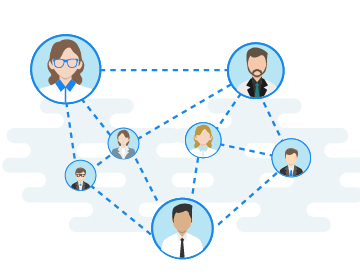
\includegraphics[scale=0.5]{SocialNetwork}
\caption{{\bf Toy social network.} A small example of a social network, with nodes being users and edges representing connections between users. Image from \url{https://www.phpfox.com}}
\label{fig:social}
\end{center}
\end{figure}

Such a network with edges simply representing whether or not a pair of nodes interact is an example of an \emph{undirected,unweighted} network. We will use an undirected network to introduce two forms of representations for networks. For a set of $N$ nodes, we define the $N \times N$ network adjacency matrix, ${\bf A}=\{a_{ij}\}$. For a pair of nodes $i$ and $j$, its corresponding adjacency matrix entry $a_{ij}$ is defined as follows,

\[ \begin{cases} 
     a_{ij}=1 & \text{\emph{if node $i$ and node $j$ are connected}} \\
      a_{ij}=0 & \text{\emph{otherwise}}.
         \end{cases}
\].

Undirected networks can also be \emph{weighted}, where the weight of an edge between a node pair encodes their extent of similarity. These edge weights are some real number and are frequently quantities such as correlation or pairwise similarity. A simple extension of ${\bf A}$ to an undirected, weighted network where $w$ is the edge weight between nodes $i$ and $j$ computes the adjacency matrix entry $a_{ij}$ as, 

\[ \begin{cases} 
     a_{ij}=w & \text{\emph{if node $i$ and node $j$ are connected} with weight $w$} \\
      a_{ij}=0 & \text{\emph{otherwise}}.
         \end{cases}
\]

Alternatively, the assumption of a symmetric relationship between a pair of nodes that node $i$ connects to node $j$ and node $j$ connects to node $i$  may be unrealistic. For example, on twitter, user $i$ can follow user $j$, but user $j$ does not necessarily need to follow user $i$. This type of network is known as a \emph{directed} network. While directed are frequently discussed in the network science literature, we will not introduce them here.  

\subsection{Network Summary Statistics}
Given a network, there are fundamental tasks of interest that allow for a more clear interpretation and understanding of the data. Some of these objectives include, quantifying node importance, quantifying edge density, identifying connected components ,clustering nodes, and predicting links. Networks in textbooks often look deceptively clean and well-structure. In reality, most network data is described as being a hairball. This term refers to the difficulty of discerning structure or interpreting meaning from the network based on the connectivity patterns. An example of a typical hairball is shown in figure \ref{fig:Hairball}

\begin{figure}
\begin{center}
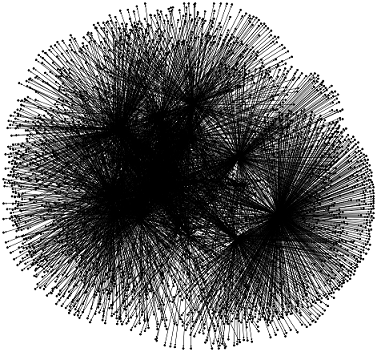
\includegraphics[scale=0.3]{Hairball}
\caption{{\bf Hairball network.} Networks are often noisy data structures and lack an immediate straight forward structural interpretation. Image from \url{https://cs.umd.edu}}
\label{fig:Hairball}
\end{center}
\end{figure}

Such a challenging representation of the data requires breaking the network down into smaller pieces that can be further analyzed. The first most basic summary statistic is known as \emph{degree}. Here, we will define a variety of summary statistics and quantities that can be computed on a network that give insight into the network's structure. Given the adjacency matrix for an undirected network, ${\bf A}$, the degree of node $i$, $\text{degree}(i)$ is computed as,

\begin{equation}
\text{degree}(i)=\sum_{j}a_{ij}
\end{equation}

In the case of an undirected, unweighted network, the degree of node $i$ counts its number of neighbors, while in the undirected, weighted context, degree encodes the total edge weight incident to node $i$. Collectively examining the distribution of degrees for a network is known as the \emph{degree distribution}. Understanding the degree distribution provides insight into the network type and structural organization. [Add some example maybe]. To concisely summarize this information, one may consider. ... blah blah to add. Finally, clustering on a network or identifying a partition of nodes into groups or `communities' based on structural network patterns is known as community detection. This is a powerful way to segment a network into smaller structures that can be further prioritized for additional analysis. 

\section{Conceptual Overview of Community Detection}
A community in a network is broadly defined as a set of who share something in common in terms of their connectivity patterns in the network. One can think of a community as a clustering problem on networks, where the objective is to identify a set of nodes that are highly similar. The most basic type of community to understand is a network with assortative community structure. In this case, nodes are tightly connected to each other but more sparsely connected to the rest of the network. An example of a network with assortative community structure is shown in \ref{fig:Assort.} Communities in the network are outlined with pink dotted lines.

 \begin{figure}
\begin{center}
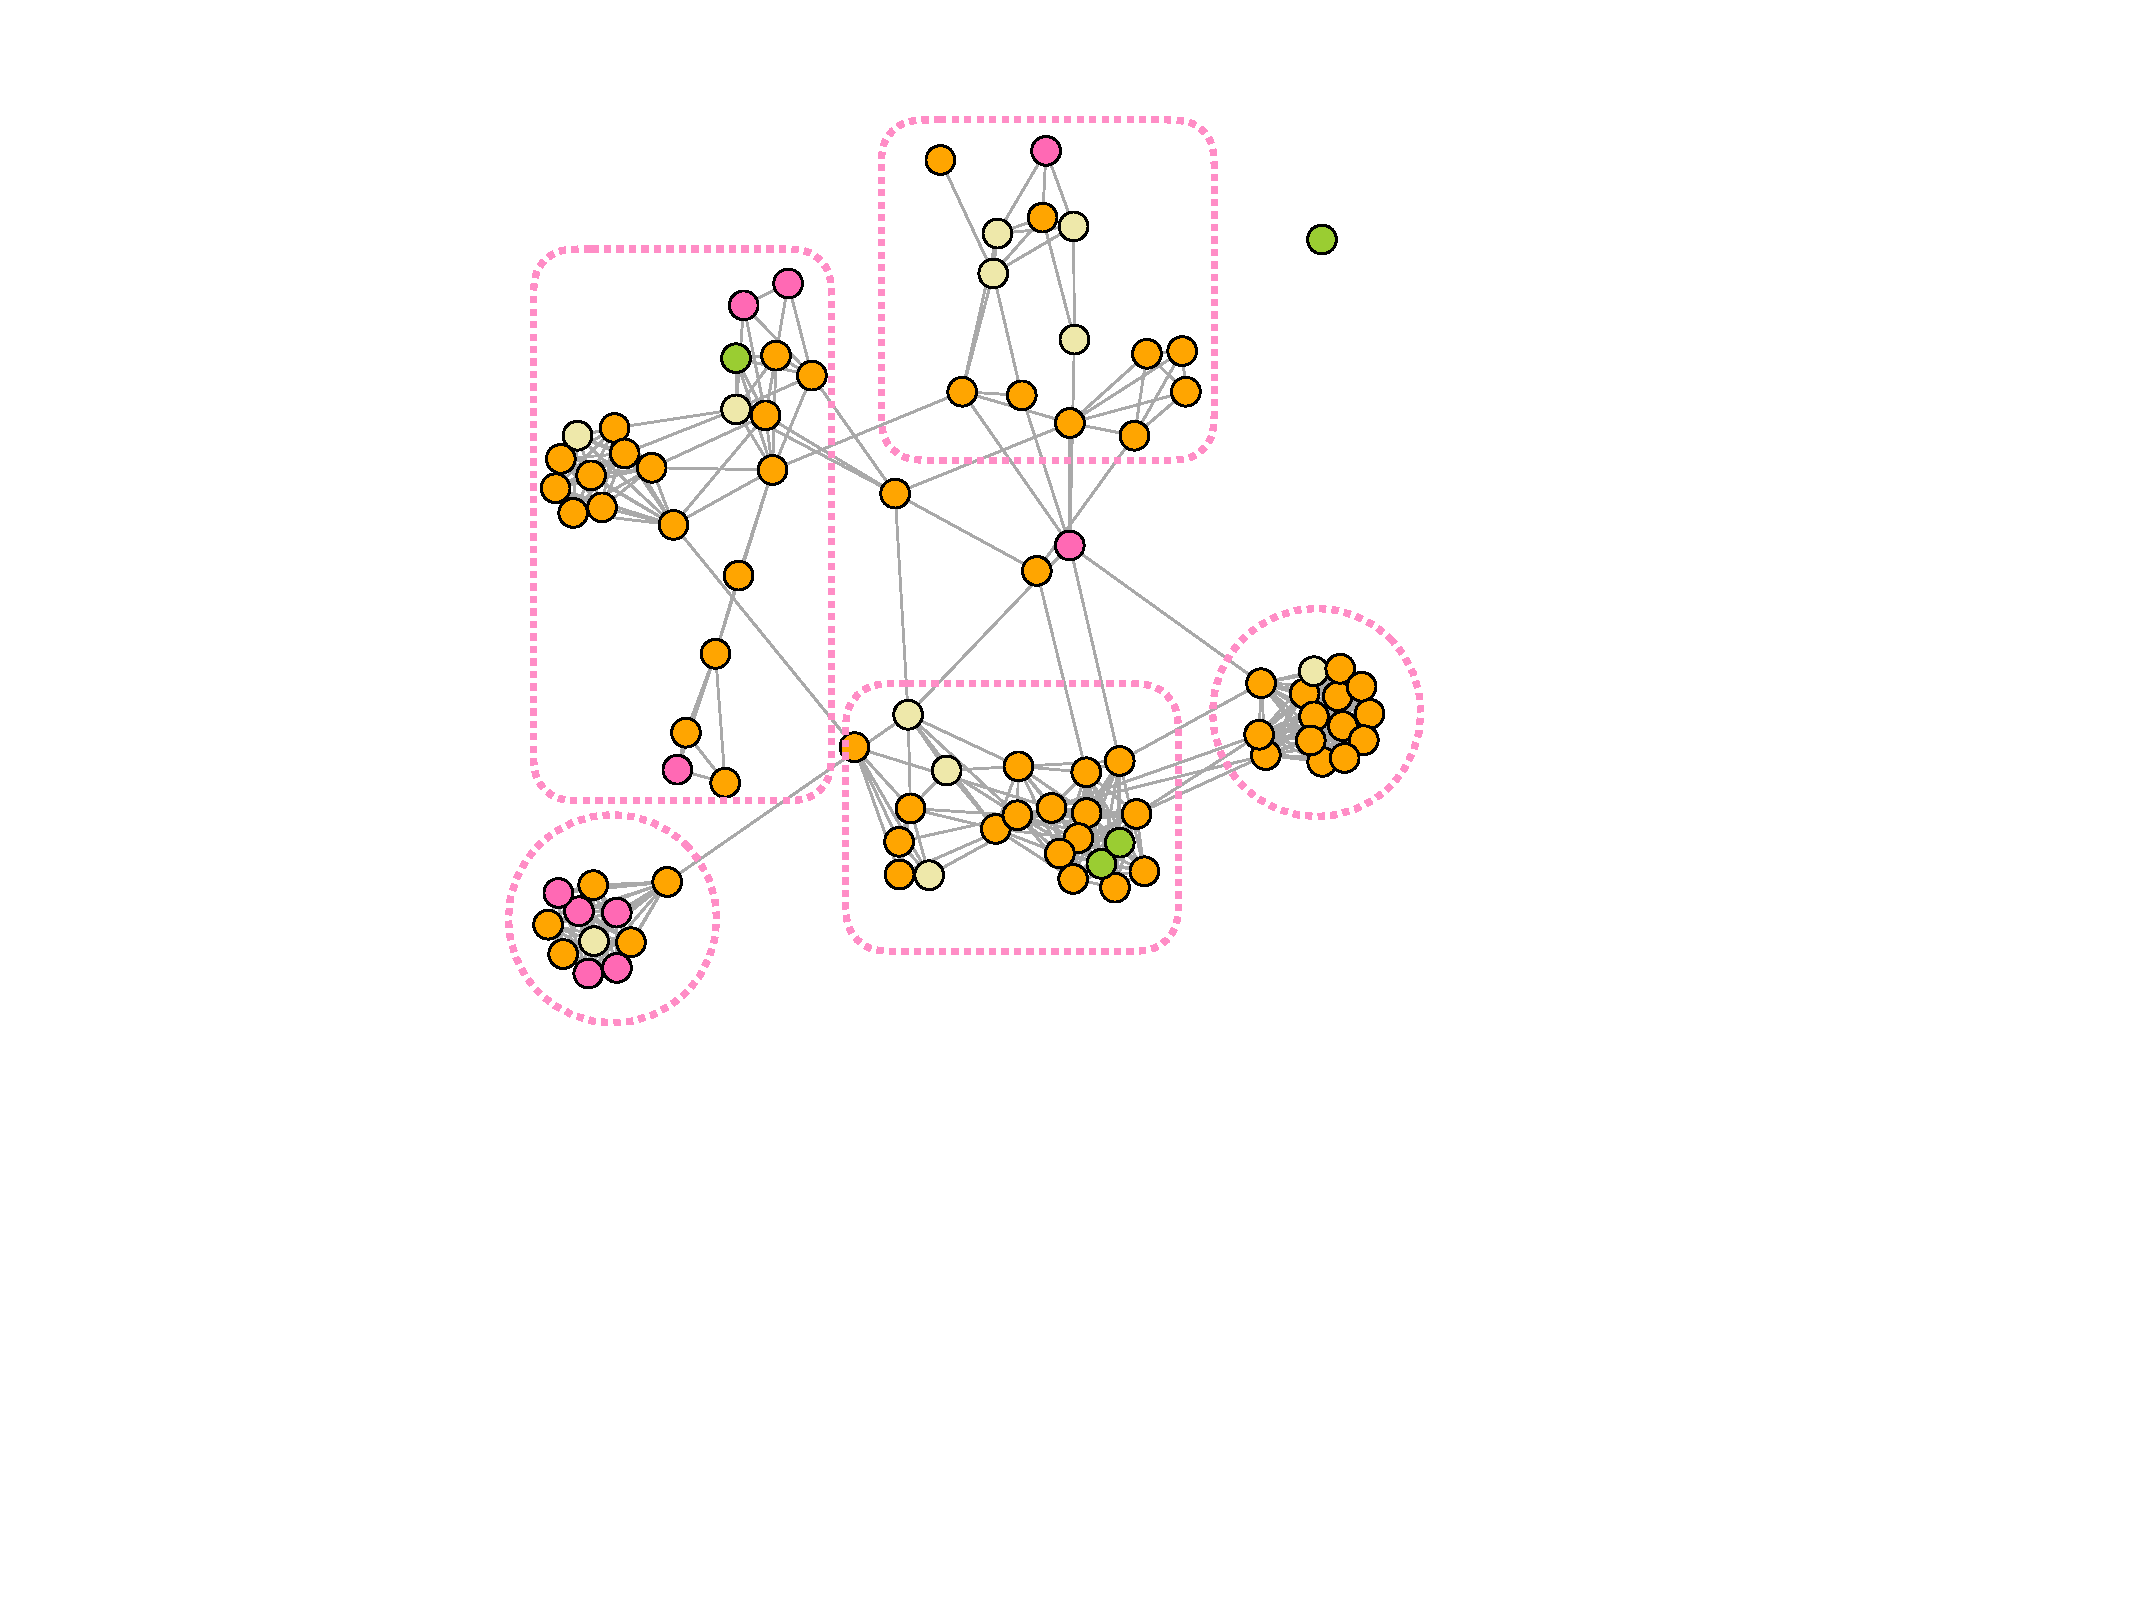
\includegraphics[scale=0.4]{AssortativeNet}
\caption{{\bf Assortative Community Structure.} Nodes are tightly connected to each other and more sparsely connected to the rest of the network. Each community is outlined with a pink dotted line.}
\label{fig:Assort}
\end{center}
\end{figure}

Alternatively, networks can have a dissasortative structure where the between community edge density exceeds the within-community density. Finally, a core periphery structure can arise when there is a central core in the network that connects to the rest of the network and a set of peripheral nodes that connect to the core, but not to each other.  

Community detection is a well-studied sub-domain of network science. The interested reader can refer to one of the comprehensive review articles \cite{fortu1,fortu2,shaicase}

\section{Introduction to community detection}
When performing community detection on a network, the objective is to segment nodes into one of $K$ communities. This $K$ can be known apriori or estimated through some kind of model selection or quality function computations. There are many optimization approaches that can be used to approach network community detection. In this section, we will introduce the current state-of-the-art approaches characterized as quality function maximization, deep learning, higher order clustering, probabilistic, and spectral methods. These methods are discussed based on their ability to handle networks of non-trivial size with diverse structures.

\subsection{Quality function maximization with modularity}
\indent For quality function optimization, one writes down a quantity to optimize that seeks to identify a partition of the network into nodes that is representative of the network structure. The most common quality function for this task is known as modularity \cite{newman2006modularity}. Intuitively, modularity defines a null model for network that doesn't have prominent organizational structure. In particular, this null model is a random graph model, known as the configuration model \cite{benderCanfield}. To generate an $N$-node network from the configuration model, one first specifies a fixed degree sequence, $D=\{k_{i},k_{2},\dots,k_{N}\}$. From this sequence, nodes are connected with $k_{i}$ stubs that will ultimately be connected together. Finally, the graph is constructed by randomly choosing pairs of the crreated stubs and joining them. Based on how this network was generated, it is easy to specify the probability that an edge exists between a pair of nodes, $i$ and $j$, or $p(a_{ij}=1$.

\begin{equation}
p(a_{ij}=1)=\frac{k_{i}k_{j}}{2M}.
\end{equation}

Here, $k_{i}$ and $k_{j}$ represent the number of edges for nodes $i$ and $j$, respectively, and $M$ is the total number of edges in the network. 

\indent Modularity was introduced in 2004 by Newman and Girvan \cite{newmangirvan}. We define the modularity quality function, $Q$ as,

\begin{equation}
Q=\frac{1}{2M}\sum_{i,j}\left[a_{ij}-\gamma \frac{k_{i}k_{j}}{2M}\right]\delta(z_{i},z_{j})
\end{equation} 

Here, $\gamma$ is a resolution parameter \cite{resParam} that controls the scale of community size. Large values of $\gamma$ favor more small communities while smaller value enforce for fewer large communities. 

\indent In order to determine ${\bf z}$, the most computationally efficient approach is known as the Louvain algorithm \cite{blondel}. The Louvain algorithm is an agglomerative heuristic, which initially starts with each node in its own community and in the first match merges pairs of nodes if their merge leads to an increase in modularity. Each group of nodes assembled after this first pass becomes a new node in the network and a new weighted network is created between the set of new nodes. The weight on the edges of the new network are the number of edges from the original network that go between the sets of merged nodes. This process is continues iteratively until the modularity no longer increases. The reason that this approach is so computationally tractable is because the gain in modularity, $\Delta Q$ of merging two groups of nodes can be explicitly computed in closed form.

\indent Modularity has shown to be effective in applications from neuroscience \cite{hierarchicalmod} to image segmentation \cite{browet}.

\subsection{Identifying communities with probabilistic approaches}

\indent This approach will be only briefly introduced here, as it will be explored more in depth in subsequent chapters. Probabilistic community detection methods aim to find a partition of the network through likelihood optimization. Intuitively, the goal is to study the generative process of the node edges in terms of inferred community assignments. For example, given nodes $i$ and $j$, one may model $P(a_{ij}=1)$ as $g(z_{i},z_{j})$, where $g(\cdot)$ is some rule based on the node-to-community assignments. Two common probabilistic community detection models are the stochastic block model \cite{originalSBM} and the affiliation model \cite{affil}. The definition and description of these models and inference techniques are described in depth in chapter \ref{probTech}.

\subsection{Deep Learning Approaches}
\indent In recent years, deep learning has begun to revolutionize many fields, including network analysis. Perozzi \emph{et al.}, pioneered the use of deep learning in community detection with the development of DEEPWALK \cite{deepWalk} to learn a latent space representation of nodes in a lower dimensional space (i.e. an emedding). Once the network is embedded in a lower dimensional space, simple clustering techniques, such as $k$-means \cite{kMean} can be used to partition the network into communities. The approach to learn an embedding for the network is based on random walks on the network \cite{rWalk,gleichpagerank}. A random walk on a network involves choosing a starting node and traversing the network by hopping between adjacent nodes. The DEEPWALK approach seeks to learn an embedding of the nodes that preserves the sets of nodes traversed in a random walk. To do this, the authors used Word2Vec, a tool from natural language understanding that allow for the specification of a node embedding that enable accurate prediction of a word's context, given the word \cite{word2Vec}. To adapt this context to networks, a random walk is treated as a sentence and nodes are treated as a word within the sentence. Moreover, the analogous task to the problem in text data to a network is to accurately assign a probability predict a set of nodes likely to be seen with the node of interest. Moreover, this problem is solved using the same optimization approach as Word2Vec \\
\indent Based on the success of DEEPWALK, the method was followed up with Node2Vec in 2016 \cite{node2vec}. While node2vec also uses the random walk framework to specify the optimization problem, they modify how the random walk is performed to enable an embedding that captures different aspects of a potential network community. For example, one may describe a community by a set of nodes located close to each other in the network with many common neighbors and connections to common neighbors. This assumption is known as network homohpily \cite{homophily}. Alternatively, perhaps a good definition of a community is a set of networks that have similar roles in the network. This idea is known as structural equivalence \cite{structural}. For example, a grouping of nodes that take into account their degree, with the community assignments being highly related to node degree. To modify the random walk so that it leads to a model that gives flexibility in the nature of retrieved communities, the authors introduced a search bias term, which controls whether the random walk in performed in a breadth-first or depth-first search parameter. If on a random walk, the path is traversed in a depth-first search, favoring the exploration of a larger area of the network far from the source, the resulting community aligns with the homophily hyptohesis. A random walk performed in a breadth first manner that restricts the path to nodes neighboring the source and tends to capture nodes based on structural equivalence (i.e. a hub, or highly connected node). 

\subsection{Spectral community detection methods}

\subsection{Higher order network analysis}

\section{Community detection in computational biology}
 A community approach to network analysis has shown to be fruitful in particular, in the analysis of biological and brain connectivity applications. In this section, we will describe examples of analyses where the identification of communities provided insight and understanding for a scientific problem. 

Multiple experimental modalities exist that enable the collection and analysis of biological data. Understanding protein expression, gene expression, microbiome composition, metabolomic profiles, genomic mutations, and immune profiling are just a few of examples of biological data that is studied routinely for insight into human health. With most experimental platforms producing high dimensional data, it is crucial to have good tools for interpretation, visualization, and prediction. Machine learning techniques in computational biology have revolutionized prediction in healthcare and medicine. Here, we outline particular examples of how community detection lead to important biological understanding and predictive ability.

\subsection{Immunological profiling to establish a pregnancy immune clock}
A study lead by Aghaeepour \emph{et al.}, demonstrated that there is a typical timing of immunological events in a healthy, term, human pregnancy \cite{immuneClock}. Immunological profiling was performed on a training cohort of 18 women, using a technology called mass cytometry \cite{cytof} was used to quantify various features of the immune system, such as, cell type abundances, signaling activity. From this set of measured immune features, a correlation network from the training cohort to identify which immune features were potentially related or working together. Simultaneously, a regression model was training to identify immune features associated with increased gestational age. When communities were identified in the network of immune features, there were two important observations. First, immune features of the same type (i.e. cell signaling vs. cell frequency) were aligned with community labels. Second, sets of features associated with a particular gestation age often fell in the same community, indicating their synchronous activity during the pregnancy. Finally, after identifying influential nodes in their ability to predict stage in pregnancy, according to the regression model, the communities of these nodes were more closely examined to uncover further insight into the immunological mechanisms occuring throughout the pregnancy time course. 

\subsection{Uncovering differences in microbiome community structure in patients with inflammatory bowel disease}

\indent The microbiome refers to the collection of bacterial species that populate an organism's gut. Microbiome analysis has recently gained attention, as its biological implications are large for health and disease. A 2017 review article presented the idea that the development of network analysis approaches for microbiome data is under explored and has great potential for advancing biological understanding and interpretation of these data \cite{networkMicrobiome}. A network in this context is typically constructed based on some notion of co-occurence or correlation between microbial species, profiled across samples A recent example where community detection played a key role in the biological understanding was introduced in 2017 and assessed the interplay between microbial co-occurence structural organization patterns between patients with and without inflammatory bowel disease \cite{moduleMicrobiome}. Communities were identified in the healthy and diseased networks, using classic modularity maximization \cite{girvancommunity}. After identifying a community structure for each network, the similarity of these partitions was quantified with the Rand index \cite{Rand}, which showed to be statistically significant under a permutation test. This observation allowed the authors to understand that the core structure from a healthy microbiome was conserved even in diseased patients, but allowed for more careful probing of the subtle differences. First, the functional roles of the members of each community were interrogated. Some interesting co-occurence relationships within communities were identified, such as the loss of strong clustering, or association propensity between pro and anti-inflammatory species within the diseased networks. This interplay between pro and anti inflammatory species is thought to play a pivotal role in the maintenance of a healthy gut microbiome. \\
\indent Next, the authors used the community structure of each network to study the differences in node roles (i.e. importance) between the healthy and IBD networks. Within the neuroscience community, there have been numerous efforts to characterize nodes, in terms of the role they play connecting communities or as an important node within a community \cite{hub}. Nodes have the potential to be \emph{connecters}, where they have high `participation' or connections with many nodes across numerous communities. Alternatively, a node can be an intramodular hub, where it serves as a high degree node, connecting to many members of its community. After assessing the role of each node in the healthy versus IBD network, the roles of many nodes were not consistent between the two networks. Most notably, the most prominent community-connector nodes in the healthy network were lost in the IBD network. Further, there were some nodes with few intermodule connections in the healthy network, that increased their role as a connector node in the IBD case. The interrogation of nodes with a dramatic change in their role are good candidates for follow-up investigation. \\
\indent Overall, the partitioning of each network into communities allowed for a systematic comparison between the healthy and disease network and to prioritize specific species (nodes) and co-occurence patterns for further investigation. 

\subsection{Community detection for analysis of flow cytometry data}
\indent Flow cytometry allows for the the simultaneous quantitative analysis of a large population of cells within a biological sample. Typically, cells are strained with fluorochrome-conjugated antibodies which emit light upon encountering laser beams in the flow cytometry machine. This emitted light is measured and reported as a quantitative measurement of the cell. An important analysis of flow cytometry data is the ability to automatically group cells based on their similarities in light emission and quantification. While this process was historically performed manually, there has been a significant amount of work to develop computational methods that can successfully segment cell populations, automatically \cite{nimaFlow}. A network-based approach to this problem, known as SamSPECTRAL was introduced in 2010 by Zare \emph{et al.}. In this approach, the authors seek to segment a population of cells into distinct populations of cells, through the construction of a similarity network and identification of communities. In this network, the nodes are comprised of the cell types in a sample, and edges between nodes indicate the similarity between a pair of cells, based on the quantification of their emitted light. Because a high throughput biological sample could contain as many as biological points, this approach seeks to first create a smaller representation of the data, build a network on this smaller version, and ultimately segment the data this way. \\
\indent To create a network of the flow cytometry data, a large subset of data points (cells) are first sampled and denoted as `registered' nodes. The next step is to look at the collection of `unregistered nodes' and ultimately assign them to their closed registered node neighbor. Iteratively, for each registered node, denoting one of these registered nodes as $P$ the set of unregistered nodes within some defined distance $h$ become registered to $p$.  The set of unregistered nodes that were newly assigned to be registered are removed from the set of unregistered nodes. This process is repeated until there are no more unregistered nodes. Each set of nodes registered with the same label are denoted as a community (an inconvenient label, given a network will be constructed and communities will be identified). A weighted network is constructed between these registered communities with edge weights quantifying the similarity in the quantitative features (as measured with the flow cytometry machine) between a pair of a communities. Once this weighted graph is created, a spectral community detection method \cite{spectral1} is applied to segment the network into 1 of $K$ network communities. These is one final post-processing step, motivated by previous work in computational flow cytometry methods,  to combine the agglomerate a pair of network communities if members if the community show similarity greater than a predefined threshold (in terms, again, of their measured flow cytometry properties). The usefulness of this approach is that it exhibited outstanding performance on datasets containing clusters of challenging shapes. For example, overlapping clusters, non-elliptical shaped clusters, or low-density clusters. To summarize, the SamSPECTRAL method shows how network communities can be used to automate a challenging computational task and enables biologists to better study and characterize their data.  

\subsection{Understanding genetic diversity of the malaria parasite genes}
\indent Rich genetic diversity in the  \emph{var} genes of the human malaria parasite has been shown to contribute to the complexity of the epidemiology of the infection and disease. The parasite can change which of the  \emph{var} genes are expressed at any given time on the infected red blood cell, which prevents the antibody from recognizing and resisting the new protein. One diversity-generating mechanism is recombination, which is the exchange and shuffling of genetic information during mitosis and meiosis \cite{varIntro}. The ability to understand genetic diversity is complicated by inadequate tools to uncover the phylogeny, or genetic relationship between sequences resulting from recombination events, in a scalable and statistically rigorous way. The typical analyses for evolutionary data assume a tree-like relationship between events, which is unrealistic for recombination data. To address this challenge, \cite{larremoreparasite} use a novel approach: they cast their problem in terms of a collection of networks. Then, they apply community detection to each of the networks and use the properties of the communities to generate hypotheses of the mechanisms behind the recombination process. To investigate the heterogeneity and the corresponding possible patterns in recombination events across a set of 307 sequences from the \emph{var} gene, the authors restricted their analyses to 9 particular ``highly variable regions'' (HVR) within each of the 307 sequences. Then for each HVR, they constructed a network, where the nodes represented the 307 sequences and an edge was placed between a pair of nodes if they had evidence of a recombinant relationship, based on a notion of sequence similarity within the particular HVR. Communities were then identified in each of the 9 networks using a degree-corrected stochastic block model (SBM) approach \cite{degreeCorrect}.\\
\indent After identifying communities within each HVR network, the authors used two summary statistics to formulate their biological hypothesis. First, the variation of information \citep{VI} was used to compare the community assignments of nodes (i.e.\ each of the 307 sequences) across the 9 HVR networks. They observed that each network had a prominent community structure (i.e.\ far from random) and that the community assignments between networks were quite distinct. These observations motivated the hypothesis that recombination events occur in constrained ways, leading to a strong community structure, and that one should analyze HVR networks individually instead of building a consensus network that aggregates the HVR networks.  Next, they used \emph{assortativity} \cite{newmanAssort} to overlay the network structure with various known biological features of the sequences, such as  \emph{var} gene length. Specifically, assortativity quantifies the tendency of nodes of the same type (e.g. same gene length) to be connected in the network. They observed that three HVR networks had community structure correlating strongly with two biological features (i.e. nodes of the same biological label tend to group together), while three other HVR networks with highly heterogenous community structure were unaligned with any of the known biology. These observations allowed for the formulation of the hypothesis that the HVRs that are unrelated to each other also promote recombination under unrelated constraints and are responsible for fostering genetic diversity to avoid immune evasion. \\

\indent Given the ability to find communities within each HVR network and the lack of similarity in community structure between HVR networks, \cite{larremoreparasite} were able to formulate and test hypotheses for the diversity-generating mechanisms of \emph{var} genes, and this would have been difficult using standard phylogenetic approaches or without adopting a community-based perspective. The application of the stochastic block model to this task provided a statistically grounded approach for testing the plausibility of the model.

\section{Challenging problems in community detection}
\subsection{Temporal Networks}
\subsection{Multilayer networks}
\subsection{Network Comparison}
\subsection{Large Networks}
\subsection{Attributed Networks}

\section{Thesis Contribution and Outline}
In this thesis, we seek to apply and develop methods for community detection that can be applied to social and biological networks. In particular, we develop three extensions of community detection to multilayer networks, large networks, and attributed networks. For each of these three challenges, we present a method, software, and results on a variety of different networks. The thesis is organized as follows: First, in chapter 2, we present a comprehensive overview of the stochastic block model and the associated inference techniques for working with probabilistic models. In chapters 3, 4, and 5, we introduce community detection methods in multilayer networks, large networks, and attributed networks, respectively. In chapter 6, we present an application of community detection for the understanding of microbiome composition in patients with burn inhalation injury.  Finally, in chapter 7, we provide future directions for the discussed work. 


 with a deep description of probabilistic network models and inference techniques in chapter 2, a develop



%%%%%%%%%%%%%%%%%%%%%%%%%%%%%%%%%%%%%%%%%%%%%%%%%%%%%%

\chapter{Probabilistic community detection models and inference techniques}
\label{probTech}
In this section, we will present two probabilistic models for community structure, the stochastic block model and the affiliation model. 

\section{Probabilistic graphical models for statistical inference}
\label{pgm}
Probabilistic network models are one approach to community detection that seek to model edge existence based on the node-to-community assignments. In doing so, the objective is to learn the node-to-community assignments that make the structure of the observed network the most likely. In this section, we will define some useful notation and concepts  To fit a probabilistic network model to data, we will define some useful notation and concepts that help simplify writing down and interpreting the likelihood. 

Probabilistic graphical models enable efficient specification and manipulation of large probability distributions through semantic structures. Given a set of random variables, $\{A,B,C,D,E,F\}$, we seek to compute the joint distribution, $P(A,B,C,D,E,F)$. This joint distribution can be expressed with a directed acyclic graph (DAG), whose structure encodes dependencies between random variables. The DAG allows for the representation of the joint distribution in a factorized way, which is computationally useful. A DAG between the set of random variables, $\{A,B,C,D,E,F\}$ is shown in \ref{fig:DAG}. 

\begin{figure}
\begin{center}
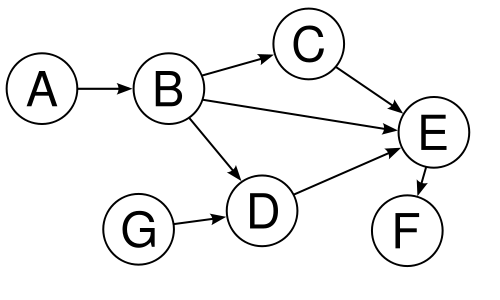
\includegraphics[scale=0.3]{DAG}
\caption{{\bf Directed Acyclic Graph.} A directed acyclic graph (DAG) is formed based on dependency between random variable and allows for a fully factorized probability distribution.}
\label{fig:DAG}
\end{center}
\end{figure}

To translate a DAG between a set of $N$ random variables, ${\bf X}={\bf X}=\{X_{1},X_{2},\dots,X_{N}\}$ to its joint distribution, we rely on the Factorization theorem, which specifies that a DAG factors according to its parent/child relationships with,

\begin{equation}
P({\bf X})=\prod_{i=1:N}P(X_{i} \mid {\bf X}_{\pi_{i}}).
\end{equation}

Here, ${\bf \pi}_{i}$ denotes the set of parents for node $i$. Using this information, we can write down the joint distribution for figure \ref{fig:DAG} as,

\begin{equation}
\begin{split}
P(A,B,C,D,E,F)&=P(A)P(B\mid A)P(C\mid B)P(D \mid B,G)P(E \mid D,B,C)P(F\mid E).
\end{split}
\end{equation}

This introduced idea will help in subsequent sections to expresses a model graphically, write down the model likelihood, and use the likelihood to optimize for the most appropriate model parameters. 



\section{Stochastic block model}
\subsection{Most general stochastic block model}
For an undirected, unweighted network $\mathcal{G}$ with adjacency matrix, ${\bf A}$, we seek to partition each of the $N$ nodes into one of $K$ communities. We denote the the node-to-community assignments as ${\bf z}$, with $z_{i}$ specifying the community assignment of node $i$. Here, ${\bf z}$ is a latent variable, with each entry taking on 1 of $K$ states, or one of $K$ community assignments. Figure \ref{fig:graphical} shows the dependency relationship between the node-to-community assignments. Here, the node-to-community assignments are treated as a latent variables because we seek to identify the ${\bf z}$ that makes the observed adjacency matrix, ${\bf A}$ the most likely.  The crucial assumption of the stochastic block model is that nodes within a community are connected to nodes within their community and to other communities in a characteristic way. To this end, the model fitting procedure requires learning a set of within and between community connection probabilities. Under this approach, edges are treated as independent and identically distributed and deciding whether or node an edge exists between a pair of nodes is the learned connection probability between the communities to which each of the nodes belong.

\begin{figure}
\begin{center}
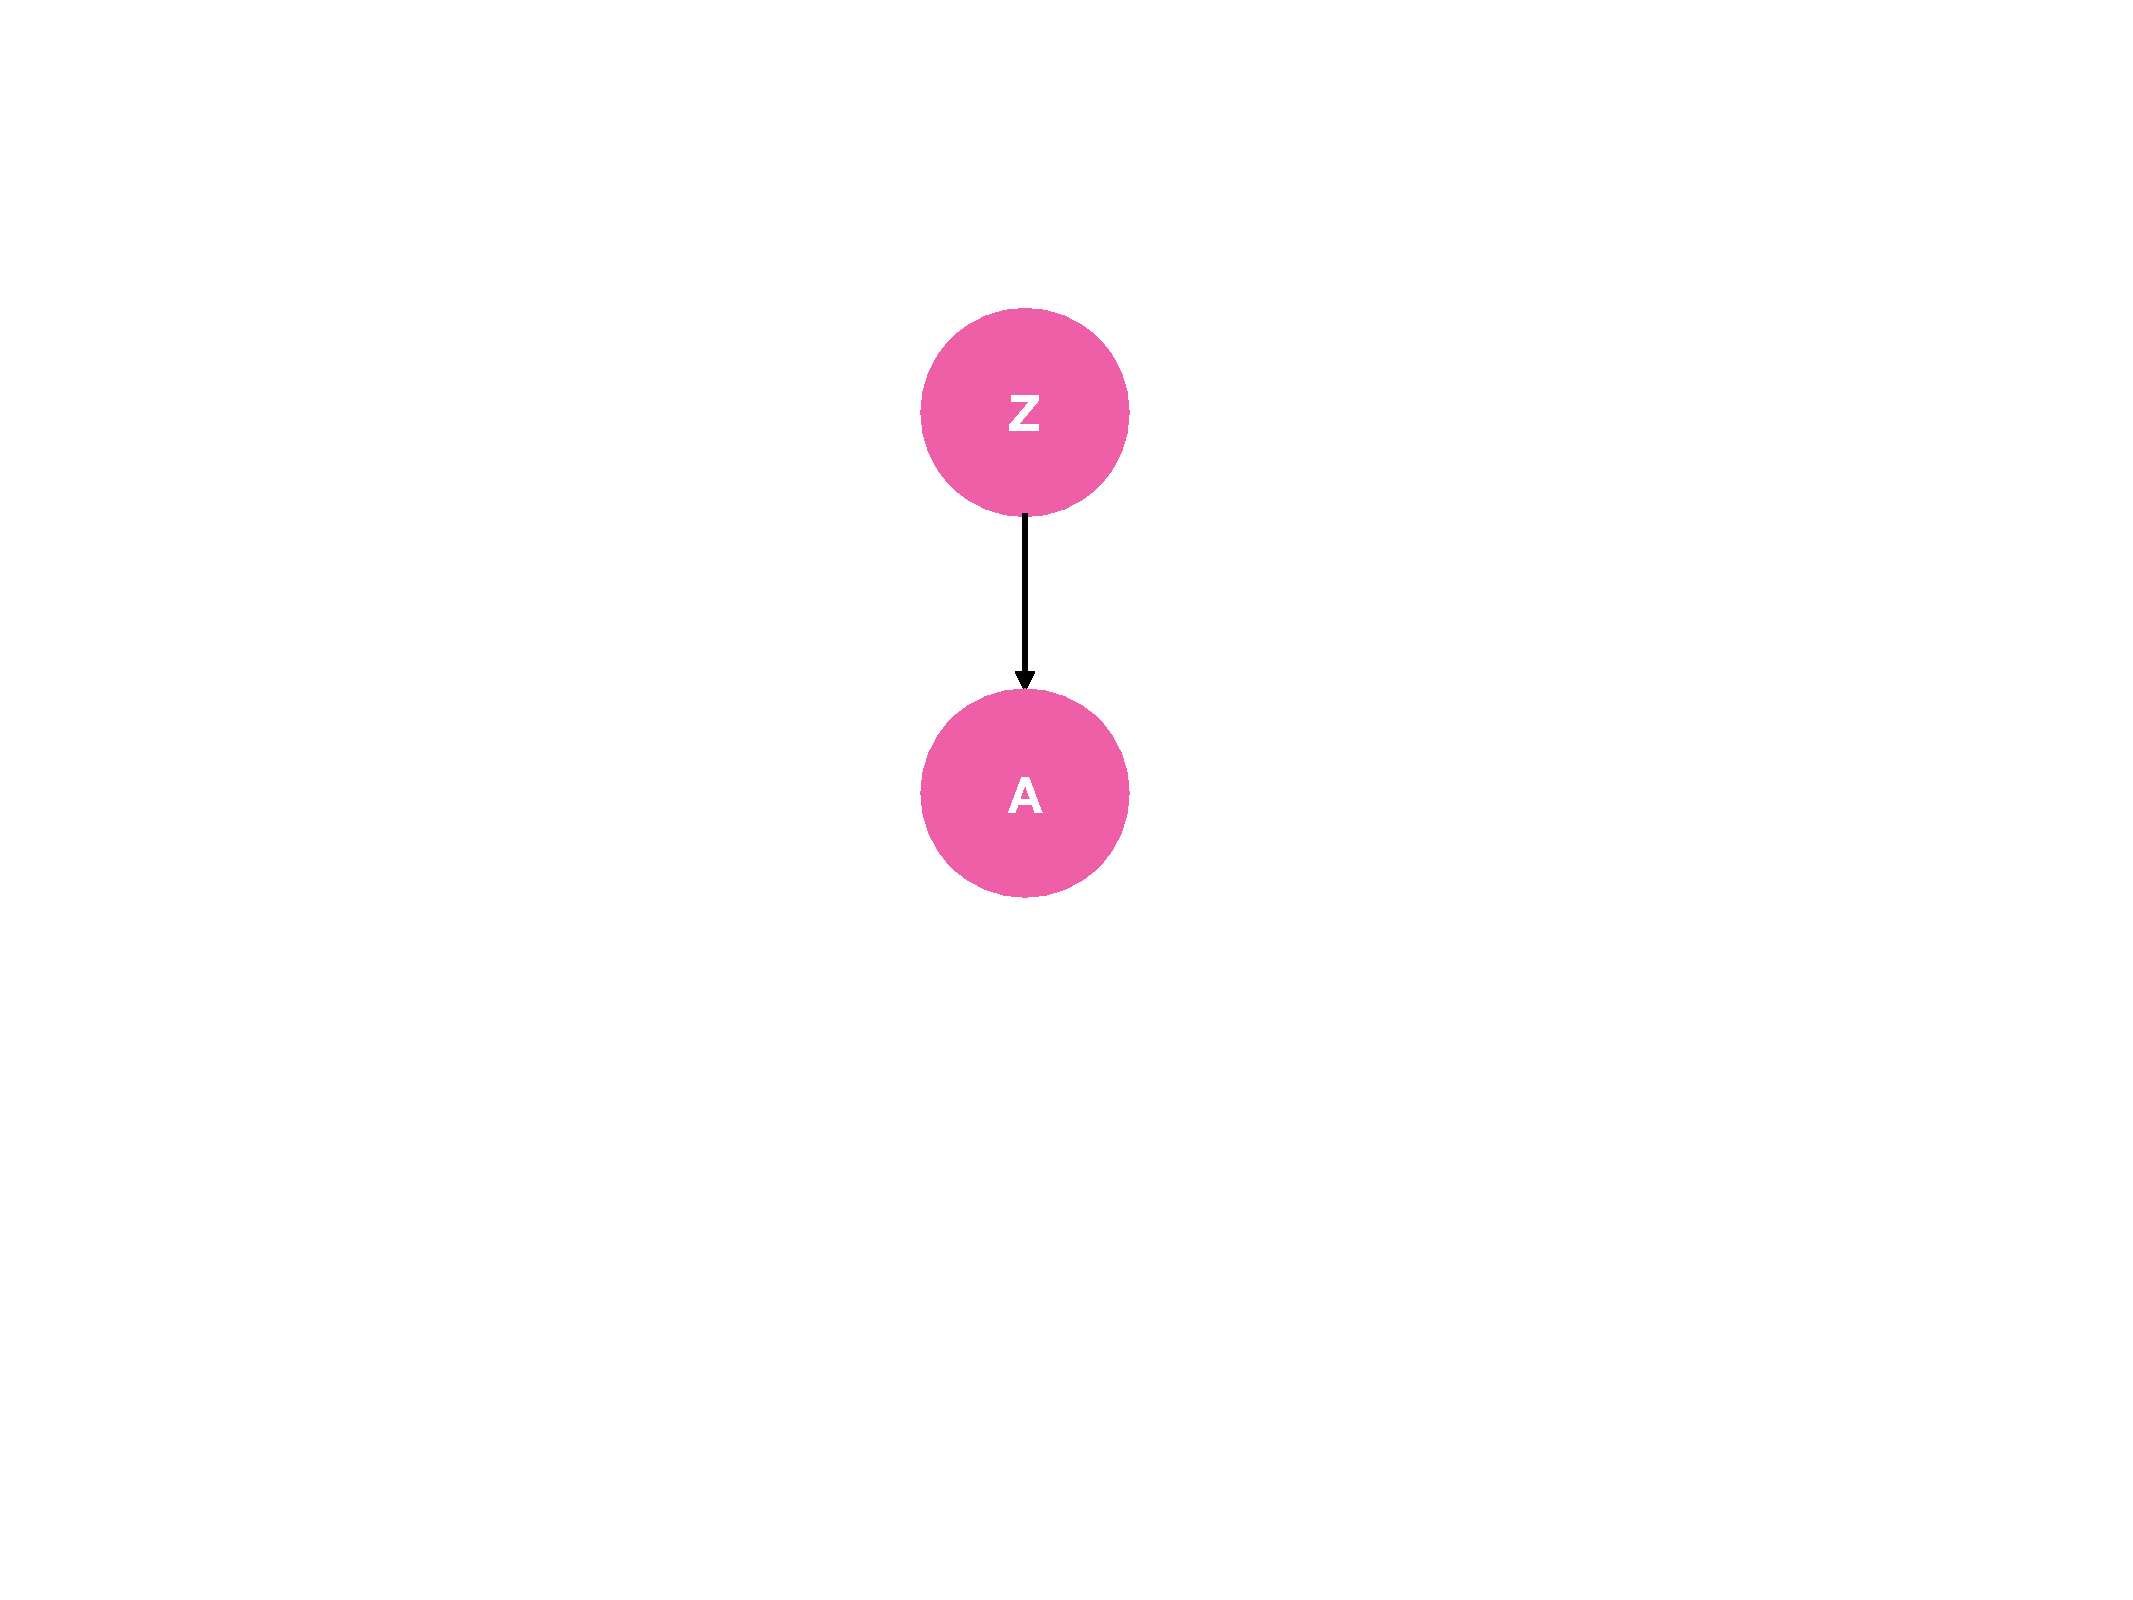
\includegraphics[scale=0.3]{SBMGraphical}
\caption{{\bf SBM Graphical Model.} A graphical model is used to model the dependency between the node-to-community assignments, ${\bf z}$ and the observed network adjacency matrix, ${\bf A}$.}
\label{fig:graphical}
\end{center}
\end{figure}

Using the factorization rules described in section \ref{pgm}, we can specify the complete data log likelihood between ${\bf z}$ and ${\bf A}$ as,

\begin{equation}
\log P({\bf z},{\bf A})=\log(P({\bf A} \mid {\bf z}))+\log(P({\bf z}))
\end{equation}

To further specify these communities, we will define additional notation. First, let ${\boldsymbol \Pi}_{K \times K}=\{\pi_{ij}\}$ be the matrix that specifies the within and between community edge probabilities. Using this information, we can model the probability of an edge existing between nodes $i$ and $j$ as,

\begin{equation}
P(A_{ij}=1)\sim \text{Bernoulli}(\Pi_{z_{i},z_{j}})
\end{equation}

We let $Z_{i}=\{Z_{i1},Z_{i2}, \dots Z_{ik}\}$ be a collection of binary indicators where $Z_{ik}$ is 1 $i$ belongs to community $k$ and 0 otherwise, We also let $\alpha_{k}$ be the probability that a node belongs to community $k$. With all of this information, we can write down each term of the complete data likelihood.

First,

\begin{equation}
\log(P({\bf Z}))=\sum_{i}\sum_{k}Z_{ik}\log(\alpha_{k}).
\end{equation}

Next,

\begin{equation}
\log(P({\bf A} \mid {\bf Z}))=\sum_{i\ne j}\sum_{k< l}Z_{ik}Z_{il}[a_{ij}\log (\Pi_{kl})+(1-a_{ij})\log(1-\Pi_{kl})]
\end{equation}

Optimizing the parameters of this incomplete data log likelihood requires computing the posterior $P({\bf z} \mid {\bf A})$ but as shown by \cite{dudin} is intractable. To address this issue, the posterior can be recast using a factorized approximation. This is accomplished by optimizing a lower bound of $\mathcal{L}({\bf A})$. We let $\mathcal{R}_{A}$ be an approximation of the posterior, $P({\bf z} \mid {\bf A})$. To optimize the lower bound of $\log \mathcal{A}$, we seek the $\mathcal{R}_{A}$ that is as close as possible to $P({\bf z} \mid {\bf A})$. In other words, we define the lower bound of $\mathcal{L}({\bf A})$ as $\mathcal{T}(\mathcal{R}_{A})$, with,

\begin{equation}
\mathcal{T}(\mathcal{R}_{A})=\log \mathcal{L}({\bf A})-\text{KL}[\mathcal{R}_{A}(\bf z), P({\bf z} \mid {\bf A})].
\end{equation}

Here KL denoted the Kullback-Leibler divergence (KL divergence) and the best approximation will be the value that makes the KL divergence the smallest. Jaakkola \emph{et al.}, present a mean field approximation for the posterior distribution \cite{jakk} as,

\begin{equation}
\mathcal{R}_{A}({\bf z})=\prod_{i}h(Z_{i};{\boldsymbol \tau}_{i}).
\end{equation}

Here ${\boldsymbol \tau}=(\tau_{i1}, \dots, \tau_{iK})$ and $\tau_{ik}$ is the approximation that node $i$ belongs to community $k$, or $P(Z_{ik}=1 \mid {\bf A})$. Furthermore, $h(\cdot;{\boldsymbol \tau}_{i})$ denotes the multinomial distribution with parameter ${\boldsymbol \tau}$. 

Daudin \cite{dudin} \emph{et al.}, show that the optimal estimate for $\tau_{ik}$ denoted $\hat{\tau}_{ik}$ satisfies

\begin{equation}
\hat{\tau}_{ik} \propto \alpha_{k}\prod_{j \ne i}\prod_{l}[\theta_{z_{i},z_{j}}^{a_{ij}}(1-\theta_{z_{i},z_{j}})^{1-a_{ij}}]^{\hat{\tau}_{ik}}.
\end{equation}

Here, $\alpha_{k}$ notes the probability that a node belongs to community $k$. Furthermore, after computing the set of variational parameters, the updates for ${\boldsymbol \alpha}$ and ${\boldsymbol \theta}$ that maximize $\mathcal{T}(\mathcal{R}_{A})$ are also shown by Daudin \emph{et al.,} \cite{dudin} to be,

\begin{equation}
\hat{\alpha}_{k}=\frac{1}{n}\sum_{i}\hat{\tau}_{ik}  \hspace{.5in}  {\theta}_{ql}=\sum_{i \ne j}\hat{\tau}_{iq}\hat{\tau}_{jl}a_{ij}/\sum_{i \ne j}\hat{\tau}_{iq}\hat{\tau}_{jl}
\end{equation}

We have presented this variational approach for performing SBM parameter inference and likelihood optimization because this approach was appropriate for the work presented in this thesis. Variational inference is just one approach that can be applied to learn model parameters and was but a study by  Zhang \emph{et al.} \cite{comp} also show that belief propgation is very effective for this task \cite{belief}. Briefly, belief propagation is a message passing algorithm for parameter inference in probabilistic graphical models. Given that parameter learning offer requires computing marginal distributions for a set of variables with a very large number of possible configurations, belief propagation uses the graphical model to reduce the complexity of the problem.  Using the belief propagation to infer latent node-to-community assignments and update the model parameters was shown to perform superperior to the variational appromixation


This formulation of the problem and parameter optimization procedure works well and converges quickly for networks that have assortative community structures and a homogenous degree distribution. We will now explore how this classic formulation of the SBM can be modified to enable a broader application for a variety of networks.

\subsection{Variants to the Classic Stochastic Block Model}

The introduced stochastic block model is the most vanilla version in that it makes the assumption that the network is unweighted, each node is assigned to only one community. The introduced model also does not account for issues that may arise from degree heterogeneity (i.e. a large disparity in node degree in sets of nodes).  Here, we will briefly discuss the approaches that adapt the stochastic block model to handle these issues and assumptions. 

{\bf Edge Weights}

\indent The majority of the stochastic block model literature considers unweighted networks simply because describing a probabilistic model to handle both edge existence and edge weight is a challenging task. In the classic stochastic block model, we are simply modeling whether an edge exists based on the inferred community memberships of the edge stubs. Since edge weights can come in a variety of forms (real-valued, count, etc.), it is difficult to immediately decide what distribution the edge weights should follow. In the past few years, this issue has been tackled in two papers \cite{aicher,peix}.

\indent First, Aicher \emph{et al.} developed a model and associated inference technique, for the weighted stochastic block model. Here, edge weights can be modeled by any exponential family distribution. The authors use a mixing parameter that allows for the control of the use of edge existence versus edge weights when learning node-to-community assignments. This method requires having an estimate of the number of communities, $K$, but the paper provides an approach to use Bayes' factors between two competing values of $K$ to determine which model is a better fit.The inference for fitting this model is performed through a variational bayes approach \cite{vBayes}.

\indent To avoid having intuition about $K$, Peixoto \cite{peix} developed a non parametric bayesian approaches that is capable of inferring $K$ with no prior knowledge. The assumption of the model is also slightly different and assumes a hierarchical structure between communities. The inference is achieved through MCMC sampling. 

{\bf Degree Heterogeneity}\\
\indent Based on the variety of network structures and types, the assumption that the classic stochastic block model is an appropriate model for the data is often invalid. That is, for some networks, the fitted model may not actually be a good fit for the data. Work by Karrer \emph{et al.}, introduced a simple extension to the classic stochastic block model, known as the degree corrected stochastic block model, that is informed by degree distribution as a proxy for the network structure. In networks where there is a high disparity between node degree (i.e. many high degree nodes and many low degree nodes), stochastic block models inference tends to partition the nodes intro communities of high degree and low degree nodes. The approach for adapting the SBM to this setting is to learn a $K \times K$ matrix, ${\boldsymbol \theta}$, describing the number of edges between each pair of communities. these counts are modeled as poisson random variables. The likelihood of the observed network under this poisson assumption takes into account node degrees. 

{\bf The restriction of single community membership}\\
\indent As it is often observed in social networks, the assumption that every node belongs to only a single community is restrictive. To address this issue, approaches have been developed to  allow nodes to  participate in a mixture of communities \cite{mixMember} or to overlapping groups \cite{LA}. Airoldi \emph{et al.}, pioneered the development of the mixed membership stochastic block model \cite{mixMember}, where instead of modeling a node's membership in each community in a binary manner, the authors allow a node to belong to multiple communities. The generative process for this approach for modeling the existence of an edge between nodes $p$ and $q$ in a network with $K$ possible communities and ${\boldsymbol \theta}$ representing the between community connection probabilities.

\begin{itemize}
\item For each node $p$, draw a mixed membership vector $\pi_{p}\sim \text{Dirchelet}({\boldsymbol \alpha})$
\item Then for each pair of nodes $(p,q)$, draw ${\bf z}_{p\rightarrow q} \sim \text{Multinomial}(\pi_{p})$, ${\bf z}_{q\rightarrow p} \sim \text{Multinomial}(\pi_{q})$
\item Sample the edge between $p$ and $q$ as, $A_{pq}$, where $A_{pq} \sim \text{Bernoulli}({\bf z}_{q\rightarrow p}^{T}{\boldsymbol \theta}{\bf z}_{q\rightarrow p})$
\end{itemize} 

Following the development of the mixed membership stochastic block model, Latocuhe \emph{et al.} \cite{LA} addressed an important limitation of \cite{mixMember}. Since the probability of an edge between a pair of nodes $p$ and $q$ depends on a single draw of ${\bf z}_{p\rightarrow q}$ and ${\bf z}_{q\rightarrow p}$, the class memberships of nodes $p$ and $q$ towards other nodes in the network are ignored. Moreover, this model adapts the mixed membership stochastic block model to incorporate more structures of the network. 

\section{Affiliation model and inference}


Duis autem vel eum iriure dolor in hendrerit in vulputate velit esse molestie consequat, vel illum dolore eu feugiat nulla facilisis at vero eros et accumsan et iusto odio dignissim qui blandit praesent luptatum zzril delenit augue duis dolore te feugait nulla facilisi. Lorem ipsum dolor sit amet, consectetuer adipiscing elit, sed diam nonummy nibh euismod tincidunt ut laoreet dolore magna aliquam erat volutpat.   

Ut wisi enim ad minim veniam, quis nostrud exerci tation ullamcorper suscipit lobortis nisl ut aliquip ex ea commodo consequat. Duis autem vel eum iriure dolor in hendrerit in vulputate velit esse molestie consequat, vel illum dolore eu feugiat nulla facilisis at vero eros et accumsan et iusto odio dignissim qui blandit praesent luptatum zzril delenit augue duis dolore te feugait nulla facilisi.   

Nam liber tempor cum soluta nobis eleifend option congue nihil imperdiet doming id quod mazim placerat facer

\chapter{A multilayer stochastic block model}
In this chapter we present the strata multilayer stochastic block model (sMLSBM). The sMLSBM method and inference described here is described in \emph{Clustering Network Layer with the Strata Multilayer Stochastic Block Model} \cite{smlsbm}. The goal in developing this method is two-fold. First, we seek to develop an approach to cluster network layers within a multilayer network. Second, we wish to develop a novel extension to the stochastic block model to handle the information contained across network layers and determine which subsets of the network layers are are likely to be samples from the same stochastic block model. 

\section{Introduction to multilayer networks}
Currently, we are relatively comfortable working with a single network of nodes and edges, capturing one type of relational definition. We have seen this numerous times thus far in this thesis, from modeling similarity of immune features in women during pregnancy to profiling microbiome species co-occurence patterns in patients with IBS. With the consistently improving ability to generate and analyze large amount of biological data, there is often the opportunity to generate multiple relational definitions between a set of objects. This could be simply the desire to compare a gene co-expression network across multiple tissues \cite{ohmNet}, or the desire to study multiple microbial co-occurence networks in different sites of the body \cite{microbiome}. Multilayer networks provide a framework to do this, in that each relational definition leads to a new layer in the network \cite{kivelamultilayer,boccaletti2014structure,manlioMathFoundations}.  Such data and corresponding networks have shown to be useful in many contexts, such as, in the comparison of genetic and protein-protein interactions in a cell \cite{genetic}, in understanding underlying relationships and community structure across social networks \cite{socialnetwork}, and in the analysis of temporal networks \cite{muchamultislice}. Furthermore, recent advances in the mathematical foundations for multilayer networks have made analysis of these types of data more feasible. In particular, \cite{manlioMathFoundations} has introduced a mathematical formalism with tensors. Doing so allows for the calculation of important network quantities, such as centrality and clustering coefficients, as well as modularity \cite{muchamultislice}. Thus, given the inherent multiplexity of network data across fields as well as recent theoretical developments for handling these types of data, there exists a need for the development of appropriate tools that can leverage information from all layers to elucidate structural patterns.

\indent Inspired by the ideas in \cite{domen} that groups of layers often provide redundant information, we seek to further explore this idea to identify sets of layers, which we denote as ``strata", with each stratum described by a single probabilistic model based on community structure.  This effectively amounts to defining \emph{local} probabilistic network models, and is analogous to biclustering \cite{biclustering} or co-clustering \cite{cocluster} problems. Moreover, our method can be regarded as a joint clustering procedure, in which the nodes and layers of networks are clustered simultaneously. Just as in \cite{cocluster}, where the objective is to jointly cluster words and documents such that joint word-document subgroups correspond to particular topics, our objective is to cluster network layers such that each stratum is a set of layers with a characteristic community structure. To achieve this goal, we have developed the strata multilayer stochastic block model (sMLSBM). We additionally emphasize that by collectively utilizing similar layers in a principled way, we can achieve more robust community detection and parameter inference for the probabilistic community detection models that describe each stratum. 

\section{Comparing network layers based on community structure}
\indent The problem of aggregating layers in a multilayer network is closely related to the problem of clustering networks. That is, given an ensemble of networks, one aims to identify sets such that networks within a set have similar characteristics. 
These characteristics, or ``features'' in this context, can describe any of the following: micro-scale structural properties such as subgraph motifs \cite{ugander2013subgraph,motiffinding}; multiscale properties such as community structure \cite{taxonomy,NONCluster,confusingMesoscopic}, the spectra of network-related matrices \cite{structurenetwork} and by defining latent roles \cite{netensemble}. Although clustering layers in a multilayer network is closely related to clustering networks in an ensemble, these are distinct problems with different difficulties and nuances. We focus on the prior pursuit; however, we expect for certain network ensembles that it will be beneficial to modify and apply our methods to the clustering of networks. 
%These include subgraph motifs \drt{\cite{scalablemotif,motiffinding}}, community structure \cite{taxonomy}, multiscale properties such as topological summaries [dane], and network summary statistics \cite{netensemble,structurenetwork}.
\\
\indent 
In this work, we analyze and compare layers in a multilayer network based on their community structure. Community detection in single-layer networks is an essential tool for understanding the organization and functional relatedness between nodes in a network \cite{porter2009communities,fortunato}.
Although there are many definitions for what constitutes a ``community'' \cite{rombach2014core}, one often assumes an ``assortative community'' in which there is a prevalence of edges between nodes in the same community as compared to the amount of edges connecting these nodes to the remaining network. In seeking to identify such communities, numerous approaches have been proposed, including those based on
%Identifying communities in networks typically requires the identification of the best partitioning of nodes into groups to maximize number of within-community edges, which can be quantified by multiple approaches, such as 
maximizing a modularity measure \cite{newmanmodularity} and fitting a generative probabilistic model \cite{abby}. Because each of these approaches present computational challenges for efficiently detecting communities, numerous heuristics exist for developing practical algorithms \cite{community,fortunato,leskoveccommunity,clausethierarchy,newmanspectral}. \\
\indent While our approach is to define a probabilistic model for multilayer community structure, we note that there have previously been approaches to understand similarities in network ensembles that are grounded in exploiting similarities in community structure between networks. In \cite{NONCluster}, the authors seek to partition a group of networks into subgroups through construction of a network of networks (NoN). Communities in the NoN are chosen such that the networks representing the nodes are sufficiently similar in their underlying community structure. In one significant application of this method, the authors clustered gene co-expression networks and found an increased number of significant functional enrichment categories for biological processes. Similarly, in \cite{confusingMesoscopic}, the authors explore mesoscopic similarity between layers using an informational theoretic approach. While they have designed their method to handle any feature of network architecture, they highlight their ability to quantify similarity between network layers based on node-to-community assignments in the layers. \\
%
%
%In this research we compare networks based on their community structure. Specifically, 
\indent In seeking a statistically-grounded approach for studying communities in multilayer networks, we consider the stochastic block model (SBM) \cite{SBM}, a popular generative model for community structure in networks. The assumption of the SBM is that nodes in a particular community are related to nodes within and between communities in the same way, thus allowing SBMs to describe several types of communities (e.g., assortative, disassortative, core-periphery, etc. \cite{rombach2014core,aicher2015learning}). 
%
There are many other appealing aspects of stochastic block models; for example, a model-based approach allows for the denoising of networks through the removal of false edges and the addition of missing edges \cite{abby,guimera2009missing}.
%
As we introduced in chapter 2, the inference procedure for fitting SBMs to an undirected network with $N$ nodes and $K$ communities involves learning the two parameters, ${\boldsymbol \pi}$ and ${\bf Z}$. Parameter ${\boldsymbol \pi}$ is a $K \times K$ symmetric matrix, where $\pi_{mn}$ gives the probability of an edge existing between a given node in community $m$ and another node in community $n$. Matrix ${\bf Z}$ is an $N \times K$ indicator matrix, wherein each binary entry $Z_{im}$ indicates whether or not node $i$ is in community $m$. Each row of ${\bf Z}$ is constrained such that $\sum_{m=1}^{K} {Z}_{im}=1$, i.e. each node only belongs to 1 community. We also define vector $\boldsymbol z$, which has entries $z_{i}=\text{argmax}_m \{Z_{im}\}$ that indicate the community to which node $i$ belongs. For a given network, these parameters are often inferred through a maximum likelihood approach, and once learned, they provide information about the within and between community relatedness. 

\section{Related work in community detection of multilayer networks}
Due to the ubiquity of network data with multiple network layers, community detection in multilayer networks constitutes an important body of research. Important directions include generalizing the modularity measure \cite{muchamultislice} and studying dynamics \cite{manlio2} for this more general setting. 

Given the usefulness of SBMs for the understanding of node organization in single-layer networks, it is important to extend SBMs to the multilayer framework, and indeed this direction of research is receiving growing attention  \cite{airoldi,mlsbm1,barbillon,catala,thiagomlsbm}. In this context, the general assumption is that there are shared patterns in community structure across the layers of a multilayer network, and the goal is to define and identify a stochastic block model that captures this structure. These works have explored many types of applications that can arise involving multilayer networks,
%
and have therefore given rise to several complementary models for multilayer stochastic block models (MLSBMs). We now briefly summarize this previous work that is very related, but notably different, from the model we study herein.
%
%Specifically, research thus far focused on two problems: one has a given network with many layers, or one has a single layer that is assumed to be derived from some aggregation of the layers. 
\\\indent 
 In Refs.~\cite{airoldi,mlsbm1,barbillon}, the authors studied situations in which many layers follow from a single SBM. In these instances, it is possible to obtain improved inference of the SBM parameters by incorporating multiple samples from a single model. For example, in Ref.~\cite{airoldi} the authors considered an increasing number of layers, $L$, and explored asymptotic properties of the estimated SBM parameters. Specifically, they fit an SBM to each individual layer in a way that utilizes the information from all layers, and they showed convergence of these estimators to their true values as $L\to\infty$. %As expected, as the number of layers increases, so does the quality of inference. 
For a network with $L$ layers and $K$ communities in each layer, their approach requires  an estimate of the community assignment matrix ${\bf Z}^l$ and probability matrix ${\boldsymbol \pi}^l$ for each layer $l$, the latter of which involves learning $K(K+1)L/2$ parameters.To this end, the authors extended the variational approximation for approximating the maximum likelihood estimates of SBM parameters introduced in single-layer SBMs introduced in \cite{Dudin} to the multilayer setting.
\\\indent Ref.~\cite{airoldi} was followed up by Ref.~\cite{mlsbm1}, wherein the authors addressed issues that can arise for the model when $K$ and/or $L$ is large, or if the network is sparse.They proposed a modified model called the restricted multilayer stochastic block model (rMLSBM). 
In this model, instead of learning a set of $L$ independent parameters, ${ \pi}^l_{mn}$, for each pair, $(m,n)$, each entry in ${\boldsymbol \pi}$ is fully layer-dependent so as to produce a reduction in the number of free parameters. Specifically, to determine the probability of an edge between a node from community $m$ and a node from community $n$ in layer $l$, they use a logistic link function and model the probability as $\text{logit}({ \pi}_{mn}^{l})={\pi}_{mn}+\beta_{l}$. The $\beta_{l}$ is an offset parameter representing the particular layer or type of edge. In this model, it is necessary %in an $L$ layer \drt{network} with \drt{$K$} communities
to learn $K(K+1)/2+L$ total parameters. Thus, the maximum likelihood estimate for an rMLSBM is a regularized estimator.\\
\indent  Consistent with the theme of fitting a single block model to a collection of layers, Ref.~\cite{barbillon} is similar to Refs.~\cite{airoldi} and \cite{mlsbm1} in that the authors seek to leverage information from all layers by considering the joint distribution of layers. Using this, they estimated quantities such as the marginal probabilities of node assignments to communities and the edge probabilities within and between groups. An interesting aspect of their approach is that they introduce a covariate capturing the coupling between pairs of nodes. For a network with $K$ communities and $L$ layers, this requires the estimation of $(2^{L}-1)K^{2}+(K-1)$ parameters. 
\\\indent We summarize Refs.~\cite{catala} and \cite{thiagomlsbm}, which provide techniques to determine whether a single layer network is the result of an aggregation procedure in a multilayer network. In Ref.~\cite{catala}, the authors defined a version of multilayer stochastic block model and an inference procedure for assessing whether or not a single-layer network was actually obtained from an aggregation of layers in a multilayer network; they considered the 
%they considered In particular, they \drt{seeked} to infer how network layer could have been 
aggregation of layers using boolean rules. Ref.~\cite{thiagomlsbm} describes two possible generative processes for multilayer networks: the \emph{edge-covariate} and \emph{independent-layer} models. In the edge-covariate model, an aggregated network is defined in which a given edge $(i,j)$ only appears in a single layer. Aggregating the layers in a multilayer network into a single network representation combines all of the edges from each of the layers. Thus, the translation of this idea into a generative model involves choosing a layer membership for each edge and sampling edges with a probability conditioned on adjacent nodes. In the independent-layer model, layers are generated independently from each other and the only constraint is that group membership of the nodes are the same across all layers. \\
\indent While motivation to pursue this problem originated from \cite{domen}, we point out that our approach does not provide a method for aggregating layers or reducing the number of layers in the network. Instead, it can in a sense compress the network in that the learned stochastic block model parameters for each stratum can be used to generate a sample network to serve as a consensus for that stratum. 

\section{A Summary of Novel Contributions of sMLSBM}
\indent 
While the literature on MLSBMs has recently grown quickly, there is still a need for a probabilistic generative model that allows for the layers in a multilayer network to be described by multiple SBMs. To this end, we
developed a novel multilayer stochastic block model, sMLSBM, that assigns network layers into disjoint sets that we call strata, where a collection of layers in a given stratum are assumed to be samples from the same underlying generative model. Our method can be viewed as a joint clustering procedure, where we seek to group layers into strata and nodes into communities. That is, we seek to simultaneously find layer-to-strata and node-to-community assignments. 

In order to address practical applications that can involve multilayer networks with several strata, layers, communities and nodes, we introduce an algorithm that effectively partitions layers into strata and an inference procedure to learn the SBM parameters for each stratum. Importantly, these two steps---assigning nodes to communities and layers to strata---are combined in an iterative algorithm so that an improvement in community detection can lead to an improvement in the clustering of layers into strata, which can iteratively lead to further improvement in community detection, and so on.
%
\begin{figure}
\begin{center}
\label{goals}
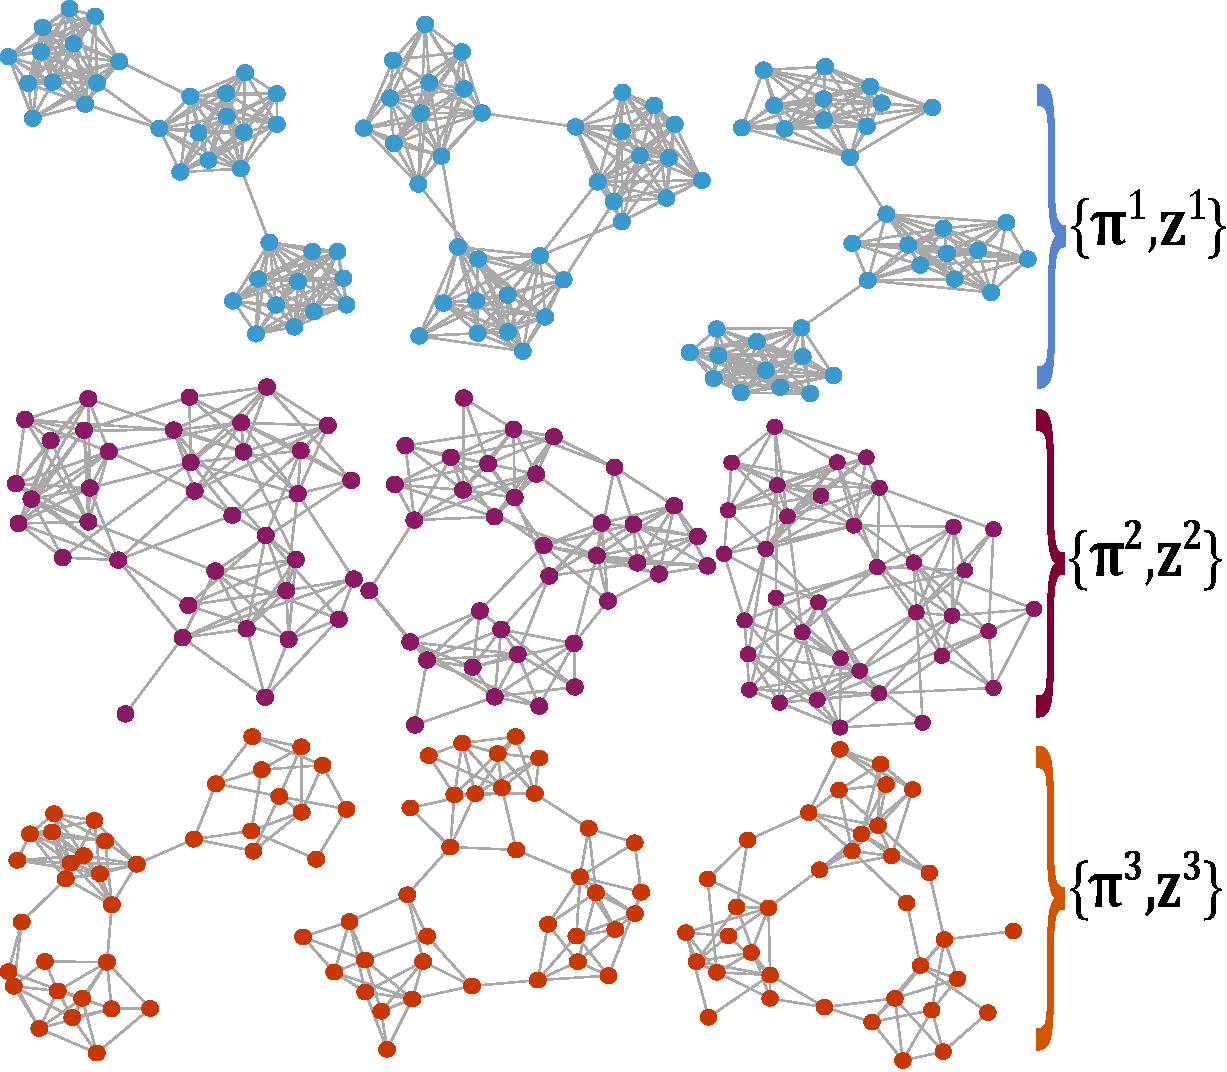
\includegraphics[width=.5\linewidth]{Figure_1.pdf}
%\includegraphics[width=1\linewidth]{FIGS
\caption{{\bf Objective of strata multilayer stochastic block model (sMLSBM)}. Each of the $L=9$ networks here represents a layer in a multilayer network. Every network layer has $N=36$ nodes that are consistent across all layers. There are $S=3$ strata as indicated by the three rows and the colors of nodes. Clearly, network layers within a stratum exhibit strong similarities in community structure. That is, although each layer follows an SBM with $K=3$ communities, the SBM parameters are identical for layers within a strata but differ between layers in different strata. We would like to partition the layers into their appropriate strata and learn their associated SBM parameters, $\pi^s$ and $Z^s$.}
\end{center}
\end{figure}

\section{sMLSBM Model Definition}
\indent Under the sMLSBM, the network layers, $G^{l}(N,\mathcal{E}^{l})$ are assumed to be generated by a set of $S$ stochastic block models, where the layers in stratum $s \in \{1,2,\cdots,S \}$, are parameterized by ${\boldsymbol \pi}^{s}$ and ${\bf Z}^{s}$ (or equivalently, vector ${\boldsymbol z}^s$, which has entries $z^s_{i}=\text{argmax}_m \{Z_{im}^s\}$ ). Note that the parameters ${\boldsymbol \pi}^{s}$ and ${\bf Z}^{s}$ for a single stratum are analogous in meaning to their respective parameters in the single-layer SBM case. 
 %
For each stratum $s$, we let $\mathcal{L}^s\subseteq\mathcal{L}$ denote the set of layers corresponding to $s$, so that $\mathcal{L}=\bigcup_s \mathcal{L}^s$ and $\emptyset=\mathcal{L}^s\cap \mathcal{L}^t$ for all $s,t\in\{1,\dots,S\}$, $s\neq t$. We let $L^s=|\mathcal{L}^s|$ denote the number of layers in strata $s$ so that $\sum_s L^s=L$.
Finally, we allow the number of communities, $K^{s}$, to vary across the strata.
\\\indent
 %Furthermore, since a stratum is composed of multiple network layers, the parameters represent a consensus for that group.
For a given multilayer network, our objective during inference is to identify the stratum assignment of each layer and to learn the collection of strata parameters, $\boldsymbol{\Pi}=\{\boldsymbol{\pi}^{1},\boldsymbol{\pi}^{2},\dots,\boldsymbol{\pi}^{S}\}$ and $\mathcal{Z}=\{{\bf{Z}}^{1},{\bf{Z}}^{2},\dots {\bf{Z}}^{S}\}$. The learned SBM parameters for a stratum represent a consensus for the associated layers, and so in that sense can be interpreted as reducing the effective number of layers \cite{domen}. However, strata can also be interpreted as a way to simply identify layers with similarities in community structure. Figure 1 shows a toy example of a multilayer network with $S=3$ strata, where each layer has $N=36$ nodes and $K=3$ communities. Each individual network in this figure represents a layer in the network. The nodes in the layers belonging to each stratum are colored according to their stratum membership; moreover, it is easy to see that layers of a stratum exhibit high similarities in community structure.  \\
  \indent As part of our procedure, we specify another parameter that we refer to as the adjacency probability matrix, ${\boldsymbol \theta}^{s}$, which can be computed from $\boldsymbol{\pi}^{s}$ and ${\bf{Z}}^{s}$. Specifically, ${\boldsymbol \theta}^{s}$ is an $N \times N$ matrix such that ${\theta}_{ij}^{s}$ gives the probability of an edge between nodes $i$ and $j$ in stratum $s$. That is, ${\theta}_{ij}^{s}={ \pi}^{s}_{z_{i}^{s}z_{j}^{s}}$, where  $z_{i}^{s}$ specifies the community number for node $i$ in stratum $s$. Finally, we define the matrix ${\bf Y}$ of size $L\times S$, wherein an entry $Y_{ls}$ is a binary indicator of whether or not layer $l$ is assigned to stratum $s$. Note that $\sum_{s}Y_{ls}=1$. We also define a vector $\boldsymbol y$, which has entries $y_{l}=\text{argmax}_s \{Y_{ls}\}$ to indicate the strata to which layer $l$ belongs.

\section{Inference for learning model parameters of sMLSBM}
\indent The procedure for fitting an sMLSBM to a given network requires finding the layer-to-strata memberships and node-to-community memberships that best describe the multilayer network. For notational convenience, we introduce hat notation to represent the learned parameter estimate from the inference procedure. We can write down the marginal likelihood for the collection of network layers, $\mathcal{G}$, as,
\begin{equation}
\label{eq1}
p(\mathcal{G}\mid {\boldsymbol \Pi})=\sum_{\mathcal Z}\sum_{{\bf Y}}p(\mathcal{G},{\mathcal Z},{\bf Y} \mid {\boldsymbol \Pi}).
\end{equation}
We assume the probability of an edge between two nodes in layer $l$ belonging to stratum $s$ can be modeled as a Bernoulli random variable, based on the community membership of the nodes. In particular, $p({A}^{l}_{ij}=1)\sim \text{Bernoulli}({\bf \pi}_{z_{i}z_{j}}^{s})$. \\
\indent Since ${\bf Y}$ and ${\mathcal Z}$ are both latent quantities, searching over all possible values quickly becomes intractable. To tackle this issue, we develop a two-phase algorithm that incorporates a clustering algorithm for choosing the best $\bf Y$. This greedy approach leads to a significant reduction for the size of the search space since only $\mathcal Z$ must be statistically inferred. Specifically, during Phase I, we infer an SBM for each layer in isolation, and we cluster together sets of layers that have similar SBM parameters. Using these results as an initial condition in Phase II, we develop an iterative method that jointly identifies layer-to-stratum and node-to-community assignments as well as the SBM parameters for each stratum. We provide a schematic of the algorithm in Fig.~\ref{fig:Schematic}, and below we present the two-phase algorithm in detail.

\noindent{\bf Phase I.}
Phase I is comprised of two parts. First, we fit an SBM to each individual layer $l\in\{1,\dots,L\}$, which yields inferred SBM parameters $\hat{{\boldsymbol \pi}}^l$ and node-to-community memberships $\hat{{\bf Z}}^l$.
Then we cluster the layers based on the similarities of $\hat{{\boldsymbol \pi}}^l$ and $\hat{{\bf Z}}^l$. To infer $\hat{{\boldsymbol \pi}}^l$ and $\hat{{\bf Z}}^l$, we use the the inference method described in \cite{Dudin}. Here, the authors used a variational inference technique to approximate the maximum likelihood estimates for the stochastic block model parameters. For the set of $L$ layers, this produces sets of SBM parameters for each layer, which we denote by $\hat{\boldsymbol{\Pi}}=\{\hat{\boldsymbol{\pi}}^{1},\hat{\boldsymbol{\pi}}^{2}, \dots, \hat{\boldsymbol{\pi}}^{L}\}$ and $\hat{\mathcal{Z}}=\{\hat{\bf{Z}}^{1},\hat{\bf{Z}}^{2},\dots \hat{\bf{Z}}^{L}\}$ (that is, at this stage of the procedure, each layer is temporarily treated as its own stratum). Note also that each $\hat{{\boldsymbol Z}}^l$ can be equivalently represented by vector $\hat{{\boldsymbol z}}^l$. Using the estimates $\hat{{\boldsymbol \pi}}^{l}$ and $\hat{{\bf Z}}^{l}$ for a given layer, $l$, we can construct the corresponding adjacency probability matrix, $\hat{{\boldsymbol \theta}}^{l}$, which is defined entry-wise by $\hat{{\boldsymbol \theta}}_{ij}^{l}=\hat{\pi}_{\hat{z_{i}},\hat{z_{j}}}^l$. Doing this for each layer results in a collection of adjacency probability matrices, $\hat{\boldsymbol{\Theta}}=\{\hat{\boldsymbol{\theta}}^{1},\hat{\boldsymbol{\theta}}^{2}, \cdots, \hat{\boldsymbol{\theta}}^{L}\}$.\\
\indent Now, we seek an initial partition of layers into strata based on $\hat{\boldsymbol{\Theta}}$. The goal is to identify $S$ sets $\mathcal{L}^s$ so that the matrices $\{\hat{\boldsymbol{\theta}}^{l}\}$ with $l\in\mathcal{L}^s$ are close to one another, but they are distant from the remaining matrices, $\{\hat{\boldsymbol{\theta}}^{l}\}$ with $l\in\mathcal{L}\setminus \mathcal{L}^s$.
%
%where the total distance across strata between the stratum consensus adjacency probability matrix and the adjacency probability matrices of stratum member layers is as small as possible. 
This is accomplished by treating each $\hat{\boldsymbol{\theta}}^{l}$ as a feature vector and applying $k$-means clustering with $S$ centers so as to identify $S$ strata, $\mathcal{L}^s$. Note that $S$ can be selected \emph{a priori}, or approximated with a measure such as the gap statistic \cite{gap}. This gives us an initial estimate $\hat{{\bf Y}}$ for ${\bf Y}$. Note that this procedure initially treats each layer as a separate stratum, but provides a principled agglomeration of layers into $S\le L$ strata.   

\begin{figure}
\begin{center}
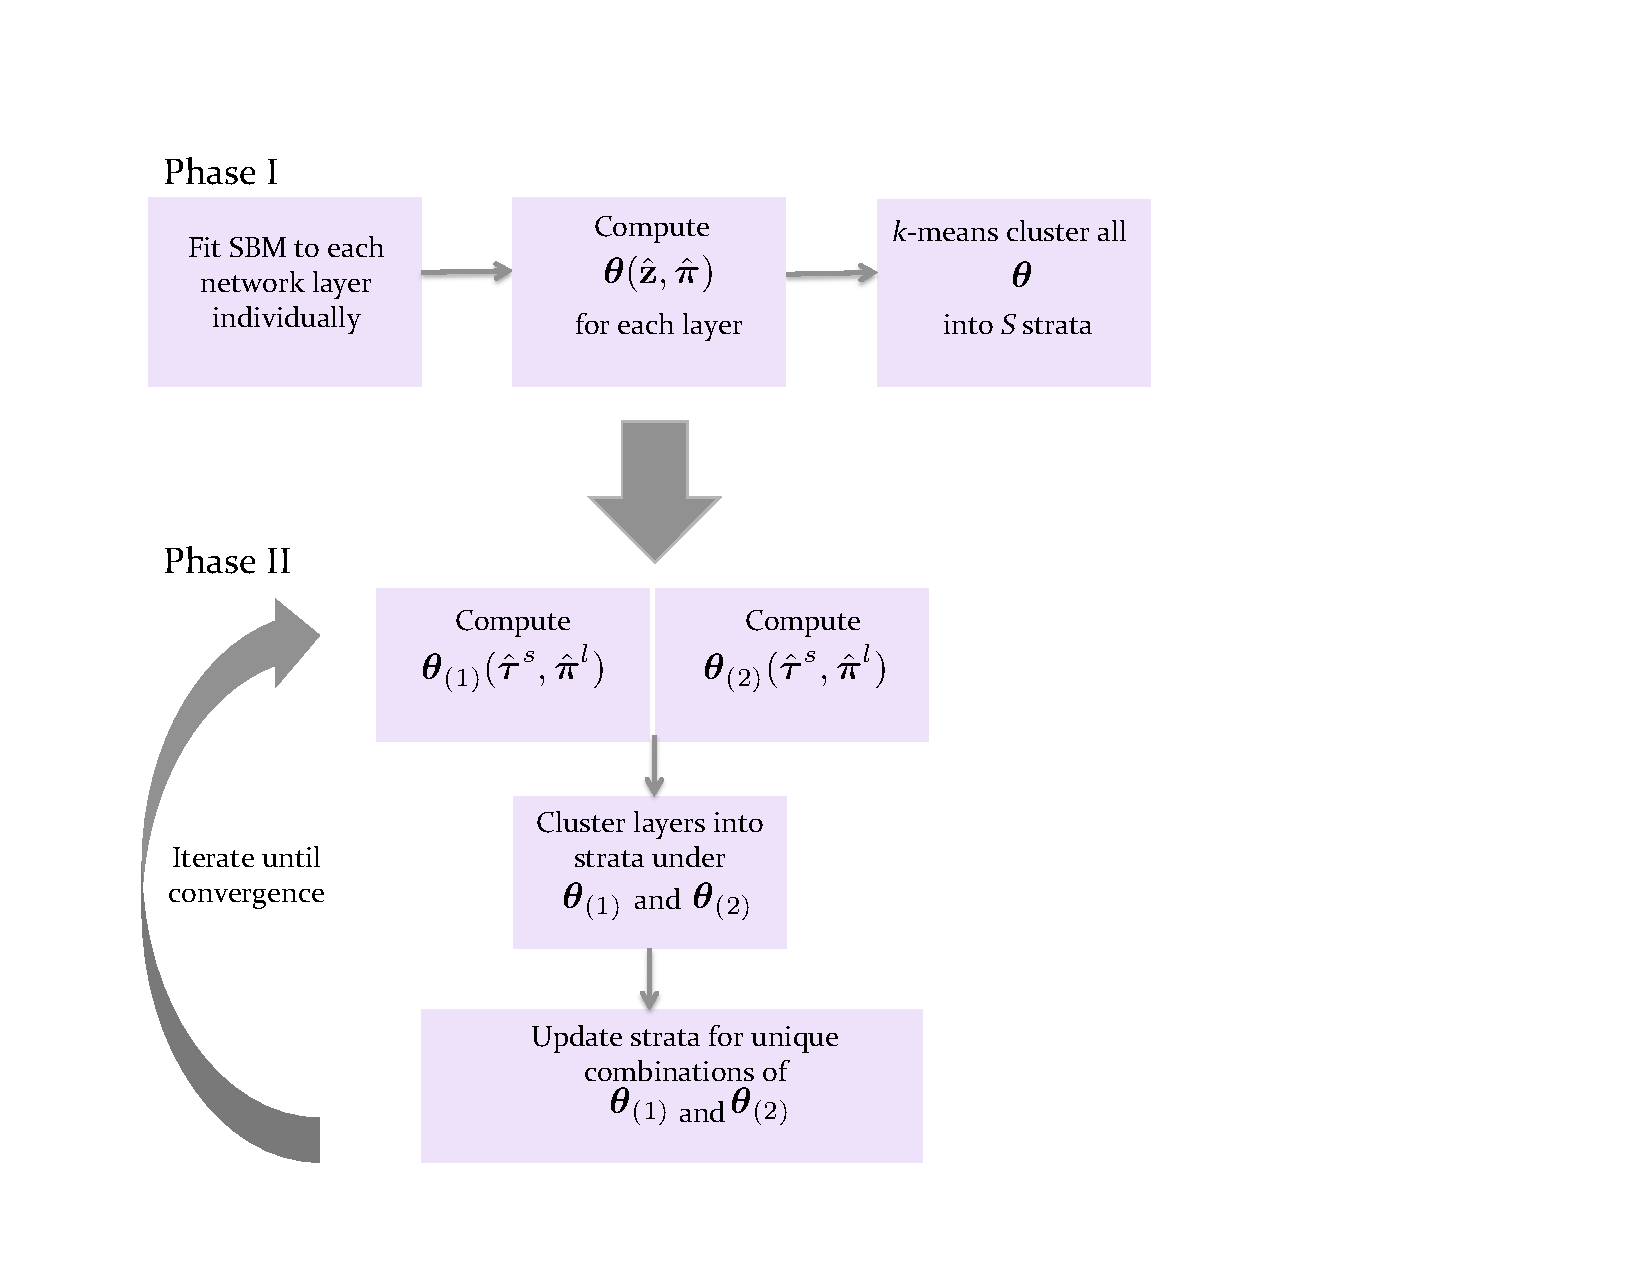
\includegraphics[width=.5\linewidth]{Figure_2.pdf}
\caption{{\bf Schematic illustration of our algorithm}: Our algorithm for fitting an sMLSBM is broken up into two phases: an initialization phase to cluster layers into strata, and an iterative phase that allows learning of node-to-community and layer-to-strata assignments.}
\label{fig:Schematic}
\end{center}
\end{figure}


\noindent{\bf Phase II.}
After a first-pass approach for assigning layers to strata, we initialize an iterative phase to more effectively estimate layer-to-strata assignments as well as the model parameters. Specifically, we would like to find the consensus SBM for each strata---that is, the $K^{s} \times K^{s}$ matrix $\boldsymbol{\pi}^{s}$ and the $N \times K^{s}$ matrix $\bf{Z}^{s}$ that maximize the likelihood of the observed layers in each stratum. We let ${\mathcal{A}}^{s}=\{{\bf A}^{l}\}$ for $l\in\mathcal{L}^s$ denote the collection of adjacency matrices corresponding to the $L^{s}$ layers in stratum $s$. 
%Hence each $\bf{A}$ is an $N \times N$ adjacency matrix. 

\indent We now proceed to maximize the likelihood in each stratum, by extending the framework of Ref.~\cite{dudin} to a multilayer context. Note that this is similar to Ref.~\cite{airoldi}, except that we are not aiming to infer an SBM probability matrix for each layer, individually. In particular, the complete-data log-likelihood for stratum $s$ can be written as,
\begin{equation}
p({\mathcal{A}}^{s},{\bf{Z}}^{s})=p({\mathcal{A}}^{s}\mid {\bf{Z}}^{s})p({\bf{Z}}^{s}),
\end{equation}
where
\begin{equation}
p({\mathcal{A}}^{s} \mid {\bf{Z}}^{s})=\prod_{l \in \mathcal{L}^{s}}\prod_{i< j}\prod_{mn}{{{\pi}}^{s}_{mn}}^{A^{l}_{ij}}(1-{{\pi}}^{s}_{mn})^{(1-A_{ij}^{l})}.\
\end{equation}
To write $p({\bf{Z}}^{s})$, it is helpful to introduce a new parameter $\alpha^{s}_{m}$ that represents the probability that a randomly-selected node in stratum $s$ belongs to community $m$, i.e. $\alpha^{s}_{m} = p({{Z}}^{s}_{im}=1)$. 

Note that $\sum_{m} \alpha^{s}_{m} =1$. 
%Further, we let $\mathcal{L}^{s}$ be the set of layers belonging to stratum $s$. 
Using this parameter, we can write
\begin{equation}
p({\bf{Z}}^{s})= \prod_{i}\prod_{m}\alpha{_{m}^{s}}^{({Z}^{s}_{im})}.
\end{equation}
%
It follows that the complete-data log-likelihood for the adjacency matrices representing the layers in stratum $s$ can be expressed as,
%
\begin{equation}
\begin{split}
\log P({\mathcal{A}}^{s},{\bf{Z}}^{s})&=\log(P({\bf Z}^{s}))+\log(P(\mathcal{A}^{s}\mid {\bf Z}^{s}))\\
&=\sum_{i}\sum_{m}{{Z}}^{s}_{im}\log(\alpha^{s}_{m})\\
&+\sum_{l \in \mathcal{L}^{s}}\sum_{i< j}\sum_{mn} A^{l}_{ij}\log({{\pi}}^{s}_{mn}) \\
&+\sum_{l \in \mathcal{L}^{s}}\sum_{i< j}\sum_{mn}(1-A^{l}_{ij})\log(1-{\pi}^{s}_{mn}).\
\end{split}
\end{equation}

Problems of this variety that involve the need to compute maximum likelihood estimates with incomplete data are typically addressed with the expectation maximization (EM) framework \cite{dempster}. Doing so requires the ability to compute $P({\bf{Z}}^{s}\mid{\mathcal{A}}^{s})$;  however, Ref.~\cite{dudin} showed that it is intractable to calculate the conditional distribution for the single-layer network case. To address this challenge, we use a variational approximation, analogous to approaches in  \cite{airoldi,barbillon,dudin}. In general, a variational approximation seeks to optimize a lower bound on the log-likelihood. To do this, we first approximate the conditional distribution, $P({\bf{Z}}^{s}\mid{\mathcal{A}}^{s})\approx{R}_{\mathcal{A}^{s}}$, where
\begin{equation}
R_{\mathcal{A}^{s}}({\mathbf Z}^{s})=\prod_{i}h({\mathbf Z}_{i\cdot}^{s};{\boldsymbol \tau}_{i\cdot}).
\end{equation}
Here, matrix ${\boldsymbol \tau}^{s}$ contains entries $\tau^{s}_{im}$ that approximate the probability that node $i$ belongs to community $m$ in stratum $s$. Further, function $h(\cdot)$ represents the multinomial distribution, with parameters, $\{{\boldsymbol \tau}^{s}_{im}\}$ for $m\in\{1,\dots,K^s\}$. Using this, we define the variational approximation as
\begin{equation}
\mathcal{J}(R_{\mathcal{A}^{s}})=\ell \ell(\mathcal{A}^{s})-\text{KL}(R_{\mathcal{A}^{s}}({\bf Z}^{s}),P({\bf Z}^{s}\mid \mathcal{A}^{s})),
\end{equation}
%
where $\ell \ell$ is log likelihood and KL is the Kullback-Leibler divergence. 

Through maximizing $\mathcal{J}(R_{\mathcal{A}^{s}})$, we minimize the KL divergence between the true conditional distribution, $P({\bf Z}^{s}\mid \mathcal{A}^{s})$, and its approximation, $R_{\mathcal{A}^{s}}({\bf Z}^{s})$. Moreover, we follow the derivation in Ref.~\cite{Dudin} and rewrite $\mathcal{J}(R_{\mathcal{A}^{s}})$ as

\begin{equation}
\begin{split}
\mathcal{J}(R_{{\mathcal{A}^{s}}})&=\sum_{i}\sum_{m}\tau^{s}_{im}\log(\alpha^{s}_{m})\\
&+\sum_{l \in \mathcal{L}^{s}}\sum_{i<j}\sum_{mn}\tau^{s}_{im}\tau^{s}_{jn}[A^{l}_{ij}\log({ \pi}^{s}_{mn})]\\
&+\sum_{l \in \mathcal{L}^{s}}\sum_{i<j}\sum_{mn}\tau^{s}_{im}\tau^{s}_{jn}[(1-A^{l}_{ij})\log(1-{ \pi}^{s}_{mn})]\\
&-\sum_{i}\sum_{m}\tau^{s}_{im}\log(\tau^{s}_{im}).\
\end{split}
\end{equation}

We can now differentiate $\mathcal{J}(R_{{\mathcal{A}^{s}}})$ with respect to each parameter---while using Lagrange multipliers to enforce constraints (i.e. probabilities summing to 1)---to compute the updates. Doing so yields the following, where the hat notation symbolizes the current best estimate for the given parameter:
%
\begin{equation}
\hat{{{\alpha}}}^{s}_{m}=\sum_{i}\hat{\tau}^{s}_{im}/N \,,
\end{equation}
%
\begin{equation}
\hat{\pi}^{s}_{qt}=\frac{\sum_{l \in \mathcal{L}^{s}}\sum_{i<j}\hat{\tau}^{s}_{im}\hat{\tau}^{s}_{jn}A^{l}_{ij}}{\sum_{l \in \mathcal{L}^{s}}\sum_{i<j}\hat{\tau}^{s}_{im}\hat{\tau}^{s}_{jn}}\,,
\end{equation}
%
\begin{equation}
{\hat{\tau}}^{s}_{im} \propto  \hat{\alpha}^{s}_{m} \prod_{l \in \mathcal{L}^{s}}\prod_{i<j}\prod_{n}[{\hat{\pi}}_{mn}^{s}{^{A^{l}_{ij}}}(1-{\hat{\pi}}^{s}_{mn})^{1-A^{l}_{ij}}]^{\hat{\tau}^{s}_{jn}} \,.
\end{equation}
%
To find the best estimates for $\hat{{\boldsymbol{\tau}}}^{s}$ and $\hat{{\boldsymbol{\pi}}}^{s}$, we alternate between updating $\hat{{\boldsymbol{\tau}}}^{s}$ and $\hat{{\boldsymbol{\pi}}}^{s}$ until convergence. When convergence has occurred, we refer to the resulting estimates as the consensus $\overline{{\boldsymbol \tau}^{s}}$ and $\overline{{\boldsymbol \pi}^{s}}$ for stratum $s$. Similarly, $\overline{{\boldsymbol Z}^{s}}$ represents the consensus indicator matrix of node-to-community assignments computed from $\overline{{\boldsymbol \tau}^{s}}$. Note that we use the bar notation to reflect that the particular parameter estimate is for a stratum, rather than for an individual layer. 

Since $\overline{{\boldsymbol \tau}^{s}}$ and $\overline{{\boldsymbol \pi}^{s}}$ are computed in terms of each other, we can use one of the consensus parameters to compute the other parameter in individual layers. 
%
In particular, using the fixed node-to-community assignments from $\overline{{\boldsymbol \tau}^{s}}$, we compute the maximum-likelihood SBM parameters  for a particular layer $l$, which we denote with a tilde and hence, $\tilde{\boldsymbol{\pi}}^l$ and $\tilde{\boldsymbol{\tau}}^l$. Similarly, for fixed $\overline{{\boldsymbol \pi}^{s}}$, we compute the node-to-community assignments $\tilde{\boldsymbol{\tau}}^l$. Such estimates allow us to determine whether or not the stratum consensus estimates are accurate estimates for the SBMs of individual layers of the stratum. 
%
More importantly, as we shall now describe, these layer-specific estimates allow us to design an iterative algorithm that allows for alternating between learning the node-to-community and layer-to-stratum assignments.

To this end, we represent each layer by the adjacency probability matrix, which we compute two different ways: letting ${\boldsymbol{\theta}}({\boldsymbol{\tau}},{\boldsymbol{\pi}})$ represent the adjacency probability matrix specified by ${\boldsymbol{\tau}}$ and ${\boldsymbol{\pi}}$, % being used to compute the adjacency probability matrix for layer $l$. Specifically, 
we define
%
\begin{equation}
{\boldsymbol{\theta}}^{l}_{(1)}={\boldsymbol{\theta}}^{l}(\overline{{\boldsymbol{\tau}^{s}}},\tilde{\boldsymbol{\pi}}^{l}) ,
\end{equation}
%
%with the ${\boldsymbol \pi}$ that provides the best match to layer $l$ using information about node-to-community assignments given by \drt{$\overline{{\boldsymbol \tau}^{s}}$.}
%
\begin{equation}
{\boldsymbol{\theta}}^{l}_{(2)}={\boldsymbol{\theta}}^{l}(\tilde{{\boldsymbol{\tau}}}^{l},\overline{{\boldsymbol{\pi}^{s}}})
\end{equation}
%
%with the ${\boldsymbol \tau}$ that provides the best match to layer $l$ using information about the stochastic block model probabilities given by ${\boldsymbol \pi}^{s}$.
Note that the first definition uses the strata-consensus estimate for ${\boldsymbol \tau}^s$ and a layer-specific estimate for ${\boldsymbol \pi}^s$, whereas the latter uses a layer-specific estimate for ${\boldsymbol \tau}^s$ and the strata-consensus estimate for ${\boldsymbol \pi}^s$.

During Phase I, we identified strata by clustering the adjacency probability matrices for the $L$ layers using the $k$-means algorithm. We employ a similar procedure here, but instead of clustering $L$ matrices, we now cluster $2L$ matrices, since each layer is represented in two different ways. Moreover, clustering these $2L$ matrices yields two cluster assignments for each layer. Typically, both representations of a particular layer will receive identical cluster {assignments---that is, for a given $l$, ${\boldsymbol{\theta}}^{l}_{(1)}$ and ${\boldsymbol{\theta}}^{l}_{(2)}$ are assigned to the same cluster, or strata. However, an interesting case arises when the two representations induce different stratum assignments for a given layer, because this implies that there is disagreement between ${\boldsymbol{\theta}}^{l}_{(1)}$ and ${\boldsymbol{\theta}}^{l}_{(2)}$, which implies uncertainty in the strata assignment of that particular layer $l$.
% ${\boldsymbol \pi}$ and single-layer ${\boldsymbol \tau}$ (and vice versa) do not have sufficient agreement. 
Because our iterative algorithm requires each layer to be assigned to a single stratum (i.e., we do not allow for mixed membership of layers into strata), layers with mixed membership according to ${\boldsymbol{\theta}}^{l}_{(1)}$ and ${\boldsymbol{\theta}}^{l}_{(2)}$ must be dealt with in some way. To account for these situations, we define additional strata for each combination of membership that arises. For example, if there are several layers $\{l\}$ that are clustered into stratum 1 according to ${\boldsymbol{\theta}}^{l}_{(1)}$ and stratum 2 according to ${\boldsymbol{\theta}}^{l}_{(2)}$, then we define a new stratum that contains only these layers. We note that there exists a variety of options for handling layers with such mixed membership after applying $k$-means clustering to ${\boldsymbol{\theta}}^{l}_{(1)}$ and ${\boldsymbol{\theta}}^{l}_{(2)}$ (e.g., one could assign such a layer to a stratum at random); however, we leave open for future work the exploration of these other options.
%the total number of partition combinations induced by the two representations of each layer determines the number of strata in the next iteration.
%\\\indent

After a single pass of Phase II, which requires layer-to-strata assignments (which can be encoded by vector $\boldsymbol y$) as input, the algorithm yields (ideally) improved layer-to-strata assignments (as well as consensus estimates for the SBM parameters of the strata, $\overline{{\boldsymbol \tau}^{s}}$ and $\overline{{\boldsymbol \pi}^{s}}$). Therefore, Phase II involves iterating the above procedure until the layer-to-strata assignments do not change. We note that in principle, it is possible for new strata to arise in each iteration (i.e., because we create strata to avoid mixed membership of layers), and this can allow the number of strata to grow with each iteration; however, we did not observe this issue in any of our synthetic or real data experiments. As we will show in the following section, convergence is typically observed after just a few iterations (e.g., see, for example, the second row of Fig.~4). If such an issue arises, it may be helpful to bound the number of iterations in Phase II. 

\section{Synthetic Examples}
Here, we demonstrate the performance of sMLSBM on synthetic networks.
\subsection{Comparison of sMLSBM to other SBM Approaches}\label{sec:SBM1}
To demonstrate a situation where the sMLSBM framework has a clear advantage over other models, we designed a synthetic experiment and compared the results to two different SBM approaches: i) fitting a single SBM to all of the layers (denoted ``single SBM''), and ii). fitting a stochastic block model to each layer individually (denoted ``single-layer SBM"). We generated a multilayer network, where each layer has $N=128$ nodes, $K=4$ communities and an expected mean degree of $c=20$ (i.e., every network layer is expected to contain $cN/2=1280$ undirected edges). We specified an sMLSBM with $S=3$ strata and 10 layers per strata, which resulted in $L=30$ total layers. We defined ${\boldsymbol \pi}^{s}$ for each stratum $s$ in terms of two parameters, $p_{in}^s$ and $p_{out}^s$, which give the within-community edge probabilities and between-community edge probabilities, respectively. That is, we define ${\boldsymbol \pi}^s_{mn}=p_{in}^s$ when $m=n$ and ${\boldsymbol \pi}^s_{mn}=p_{out}^s$ when $m\not=n$. It follows that the expected mean degree is given by $c=N(p_{in}^s + (K-1)p_{out}^s)/K$.
In our experiment, we select the following SBM parameters: $(p_{in}^1,p_{out}^1)=(0.6,0.0083)$; $(p_{in}^2,p_{out}^2)=(0.4,0.075)$; and $(p_{in}^3,p_{out}^3)=(0.125,0.167)$. 
%Because we keep $c$ fixed, this requires that $p_{out}^1=$, $p_{out}^2=$, and $p_{out}^3=$
%Given the mean degree for networks belonging to each stratum is  25, this gives corresponding values of 0.00625, 0.04375, and 0.06875 for $p_{out}$. 
In Fig.~3(A), we show an example network layer from each strata. Nodes are colored by their community assignments in stratum 1. Note that the node-to-community assignments are different in each stratum and that the extent of block structure decreases from stratum 1 to stratum 3.


\begin{figure}
\begin{center}
\label{fig:SynExp1}
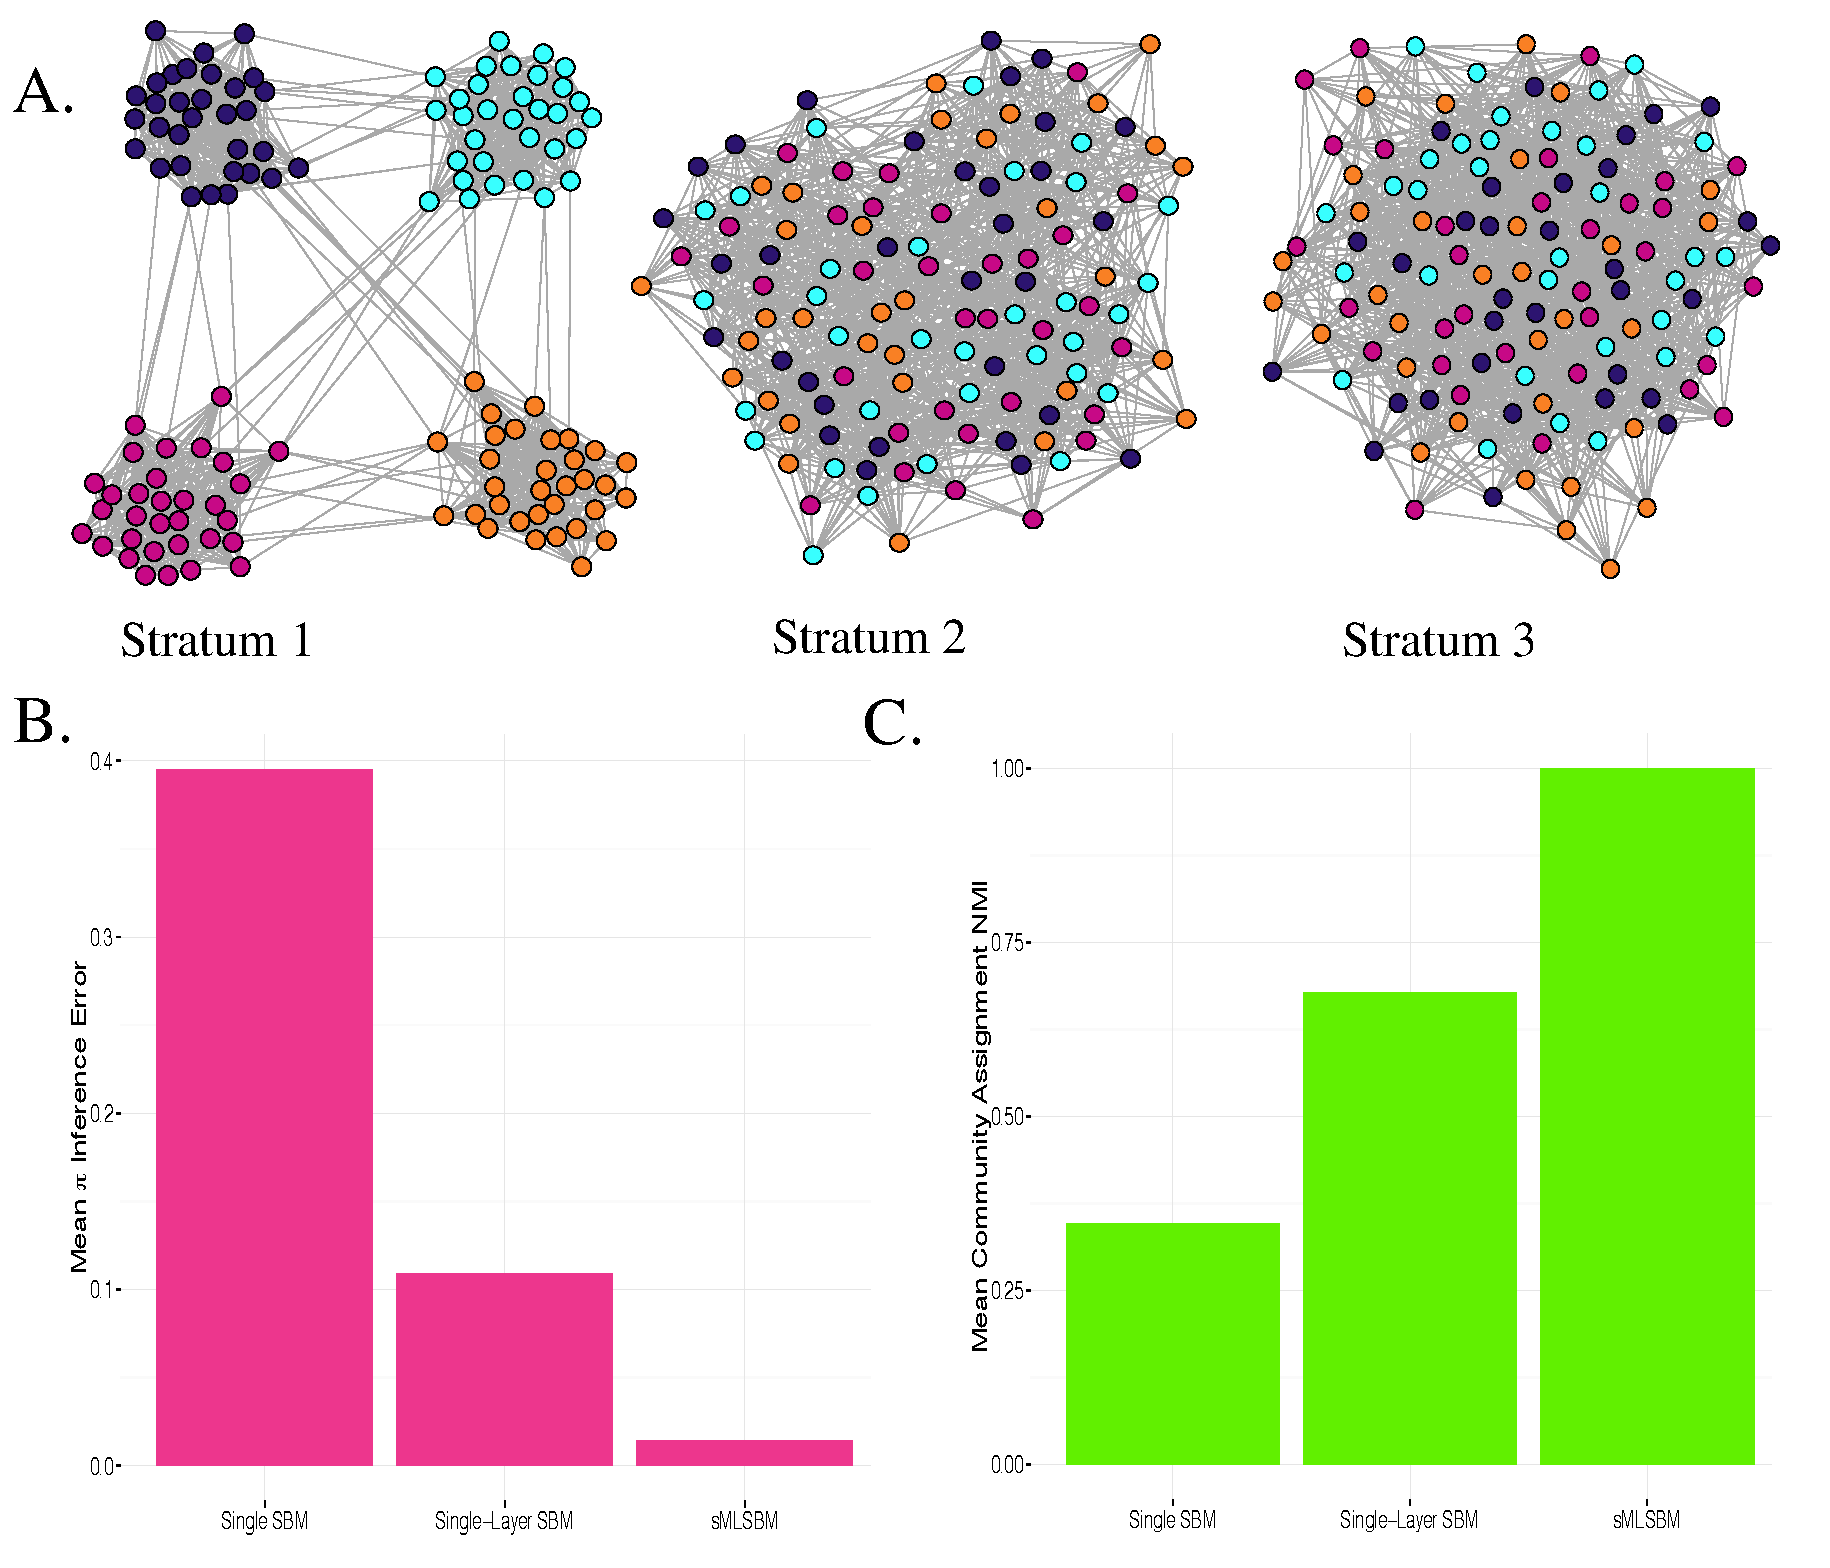
\includegraphics[width=.6\linewidth]{Figure3.pdf}
\caption{{\bf \noindent Synthetic experiment comparing sMLSBM to other SBMs.} 
%
{\bf A}.~We specified a model with $S=3$ strata and $L=10$ layers per stratum. A representative layer from each stratum is plotted. Note that nodes in all networks are colored according to their community membership in stratum 1. Each network has $N=128$ nodes, $K=4$ communities and mean degree, $c=20$. The $p_{in}^s$ parameters for $s=1,$ $2$ and 3 are 0.6, 0.4 and 0.25, respectively. Corresponding values of $p_{out}^s$ were selected to maintain the desired expected mean degree, c=20. 
%
{\bf B}. We fit 3 types of models to the 30 network layers:
i) single SBM: fitting a single SBM to all of the layers;
ii) single-Layer SBM: fitting an individual SBM to each layer; and
iii) sMLSBM: identifying strata and fitting an SBMs for each strata. 
Each model yields an estimate $\overline{{\boldsymbol \pi}^{s_l}}$ for the true SBM of each layer $l$, which is denoted ${{\boldsymbol \pi}}^{l}$. Here $s_l$ denotes the inferred strata for layer $l$.
On the vertical axis we plot the mean $\ell$2 norm error 
%between each layer's true underlying ${\boldsymbol \pi}^{l}$ and that inferred given its stratum membership $s_{l}$ under the given model. In other words, we compute, 
$||\text{vec}({\boldsymbol \pi^{l})}-\text{vec}(\overline{{\boldsymbol \pi}^{s_{l}}})||_{2}$. 
 %
 {\bf C}. For each of the three models, we computed the normalized mutual information (NMI) between the true node-to-community assignments ${{\bf z}^{l}}$ and the inferred values $\overline{{\bf z}^{s_l}}$.}
 
\end{center}
\end{figure} 

%\\\indent 
In order to compare the accuracy of fit for the three models---single-layer SBM, single SBM and sMLSBM---we quantify the inference accuracy of the SBM parameters, $\overline{{\boldsymbol \pi}^{y_{l}}}$, and community assignments, $\overline{{\bf Z}^{s_{l}}}$. 
%
First, for each layer and each model, we quantified the error ($\ell^{2}$ norm) between $\text{vec}(\overline{{\boldsymbol \pi}^{y_{l}}})$ and its true value, $\text{vec}({\boldsymbol \pi}^{l})$. Note that $\text{vec}({\bf X})$ is the $\frac{K(K+1)}{2}$ length vector representing the lower triangle of the matrix ${\bf X}$.  Moreover, to quantify error,
% parameter and the \drt{inferred parameter} $\overline{{\boldsymbol \pi}^{s_{l}}}$ under each of the \drt{three models.} 
%In other words, for each layer $l$ 
we compute $||\mbox{vec}({\boldsymbol \pi^{l}})-\text{vec}(\overline{{\boldsymbol \pi}^{s_{l}}})||_{2}$.  We note that this error is well-defined because we identify $K=4$ communities for all layers and all models. The mean error across layers under each model are shown in Fig.~3(B). In this example, sMLSBM outperforms the two other models.
%
Second, we computed for each layer the mean normalized mutual information (NMI) \cite{commdeccompare} between the true node-to-community assignments, ${\bf z}^{l}$, and the inferred values, $\overline{{\bf z}^{y_{l}}}$, under each model. In other words, for each layer, we compute, $\text{NMI}({\bf z}^{l},\overline{{\bf z}^{y_{l}}})$. Figure 3(C) shows the mean NMI for community assignments across layers. Indeed, the effects of fitting an incorrect model to a collection of layers in terms of ability to effectively estimate SBM parameters and community assignments is apparent. In particular, fitting a single SBM model results in both larger mean inference and community assignment error, compared to fitting single-layer SBMs and 3 strata sMLSBM. In other words, sMLSBM provides an efficient clustering into strata only when the layers are indeed related (i.e. generated from the same SBM), otherwise each layer is a stratum on its own.

\subsection{Synthetic Experiment with Two Strata}\label{sec:2strata}

Next, we further explored the performance of our algorithm (see Sec.~\ref{sec:Algorithm}) for inferring an sMLSBM under various situations: 1) in comparison to baseline clustering methods; 2) in response to an increase in the number of layers; and 3) under variations in levels of detectability. Specifically, we designed synthetic experiments in which we generated multilayer networks with either $L=10$ or $L=100$ layers. Every multilayer network contained $S=2$ strata (each having $K^1=K^2=4$ communities), and in each layer there were $N=128$ nodes (each having an expected mean degree of $c=16$). Note that in this example both strata have the same node-to-community assignments. The strata were fixed to be the same size, $L^1=L^2=L/2$. Similar to the experiment described in Sec.~\ref{sec:SBM1}, the SBM parameters were constructed using $p_{in}^s$ and $p_{out}^s$. Since we have already specified the expected mean degree, these parameters must satisfy the constraint $c=N(p_{in}^s+p_{out}^s)/2$ for both strata.
%
In all simulations, we fixed the SBM parameters of the first strata as $(p_{in}^1,p_{out}^1)=(.1836,.1055)$. It is also convenient to define the quantity, $N(p_{{in}}^{1}-p_{{out}}^{1})=10$, which relates to the detectability of communities \cite{decelle2011inference}. For example, the ability to detect community structure in a given layer and/or strata is, in general, expected to improve with increasing $N(p_{{in}}^{s}-p_{{out}}^{s})$. For the second strata, we allow $N(p_{{in}}^{2}-p_{{out}}^{2})$ to vary.


We present results for this experiment in Fig.~4, wherein the left and right columns give results for $L=10$ and $L=100$, respectively.

Symbols in each plot represent the mean over 50 multilayer networks, and error bars show standard error. In each plot, the vertical dotted line indicates $N(p_{{in}}^{2}-p_{{out}}^{2})=10$, which represents the point where the two strata are indistinguishable since $(p_{in}^1,p_{out}^1)=(p_{in}^2,p_{out}^2)$.
%
In Fig.~4(A), we show the NMI between the true layer-to-strata assignments and those inferred by sMLSBM, or $\text{NMI}({\bf y},\hat{\bf y})$. As a baseline, we compare sMSLBM results to directly clustering the layers' adjacency matrices using the $k$-means algorithm with $K=2$. We consistently observe higher NMI as a result of sMLSBM compared to $k$-means. More interestingly is the case with $L=100$, where both $k$-means and sMLSBM perform at least moderately well at partitioning layers into strata before the point where the strata are indistinguishable. %At this point, where the $p_{in}$ and $p_{out}$ parameters for strata 1 and 2 are the same, strata are clearly not distinguishable and we see this reflected in the drop of NMI. \\
%
In Fig.~4(B), we plot the number of iterations (NOI) required for Phase II of our algorithm to converge. We observe that as the number of layers in the network increases, so does the number of required sMLSBM iterations. Moreover, the peaks in panel B. correspond to the sudden jumps in strata NMI. 

%In both cases of $L=10$ and $L=100$, we notice a spike around when $N(p_{in}^{2}-p_{out}^{2})=20$.
%
Finally, in Fig.~4(C) we show the quality of node-to-community assignments 
%in \drt{the} strata. Particularly, we compute 
by plotting the NMI between the true and inferred node-to-community assignments as described in Sec.~\ref{sec:SBM1}. Note that stratum 1 here represents the stratum where the majority of layers were generated from model $S^{1}$ and analogously for stratum 2. Therefore, when the strata NMI is low (panel A.), we see poorer community detection results than expected, as layers get incorrectly mixed. As the strata NMI increases, layers from the same model are assigned together and the communities NMI stabilizes. 
%Specifically, we plot the mean NMI across stratum 1 (red symbols) and stratum 2 (blue symbols). As expected, we observe a general increase in NMI as $N(p_{{in}}^{2}-p_{{out}}^{2})$ increases. 
Finally, by comparing the results for $L=100$ to those for $L=10$, we observe an increase in number of layers, $L$, generally leads to an improvement in community detection and strata identification.\\


%%%%%Begin so new%%%%%%%%%%%%
\begin{figure}
\begin{center}
%\includegraphics[width=1\linewidth]{Shit}
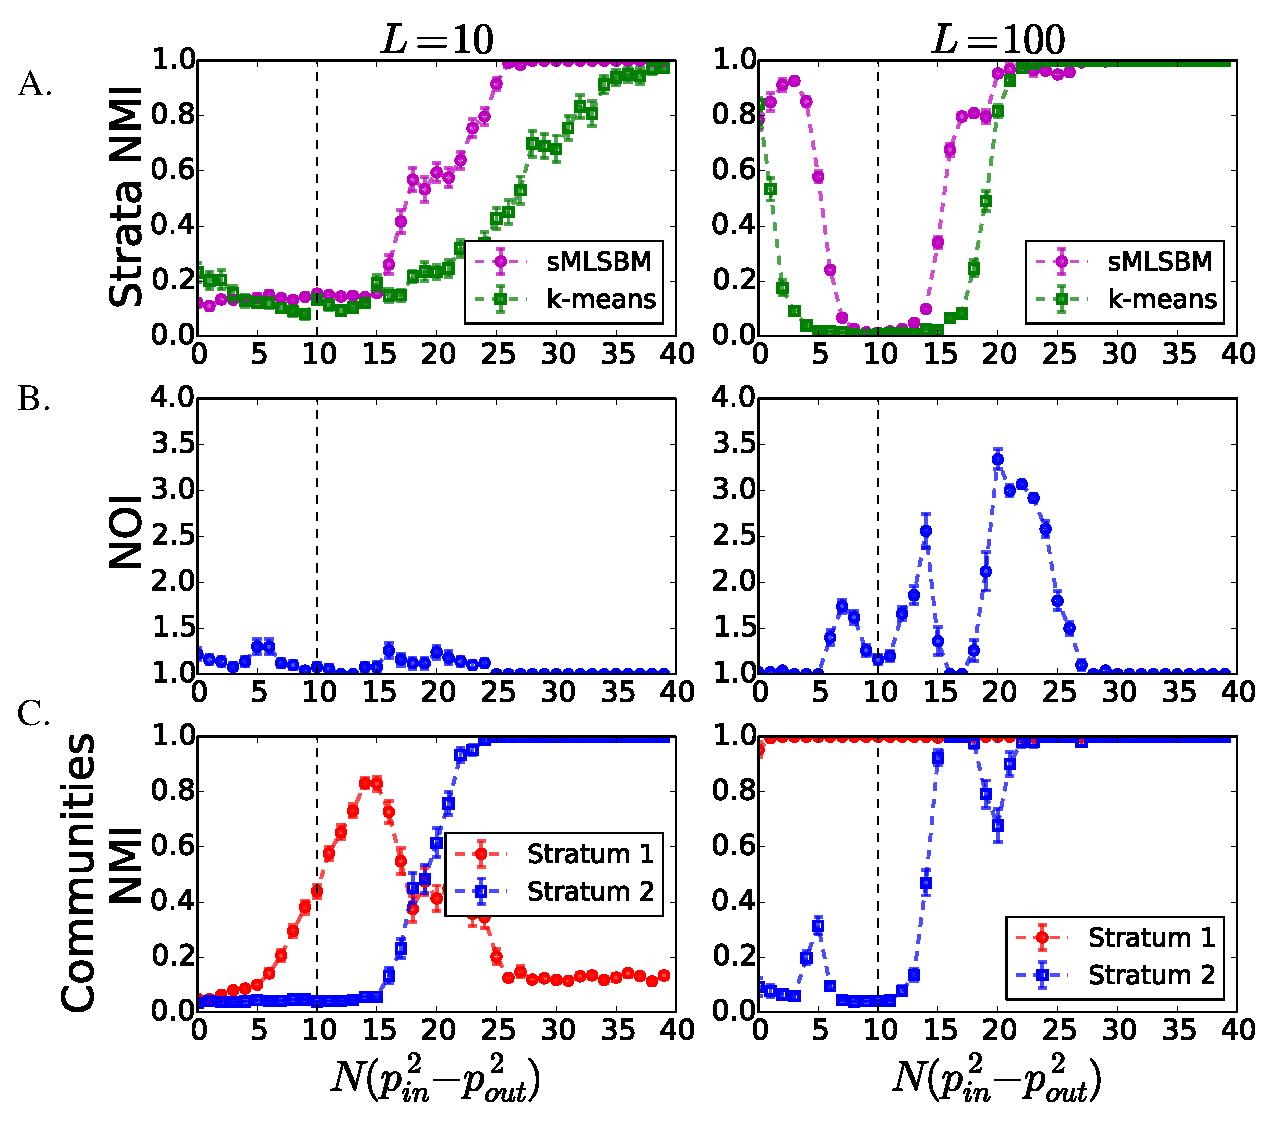
\includegraphics[width=.5\linewidth]{Figure4.pdf}
\label{fig:saray}
\caption{
{\bf Synthetic experiment with two strata.} We conducted numerical experiments with multilayer networks with $N=128$ nodes, mean degree $c=16$, $S=2$ strata and $K^1=K^2=4$ communities. The networks contained either $L=10$ (left column) or $L=100$ layers (right column), which were divided equally into the two strata. For stratum 1, we fixed the quantity $N(p_{{in}}^{1}-p_{{out}}^{1})=10$, which fully specifies $(p_{{in}}^{1},p_{{out}}^{1})$ since setting $c=16$ also constrains these parameters. In contrast, we vary $N(p_{{in}}^{2}-p_{{out}}^{2})$.
%
%Then, in each experiment we simulate 50 2- stratum networks, where the $p_{in}$ and $p_{out}$ are fixed in stratum 1, but networks in stratum 2 are generated according to $\text{Diff}_{2}$ (horizontal axis). In each plot, error bars show standard error and curves are the mean from 50 simulated networks. The vertical line in the plots shows the point at which $\text{Diff}_{1}=\text{Diff}_{2}=10$. 
{\bf A}. As a function of $N(p_{{in}}^{2}-p_{{out}}^{2})$, we plot the mean NMI to interpret the ability of sMLSBM to recover the true layer-to-strata assignments. We compare the performance of sMLSBM (purple curve) to generic $k$-means clustering (green symbols) of adjacency matrices. 
{\bf B.} We plot the mean number of iterations (NOI) required for Phase II of our algorithm to converge.
{\bf C.} Finally, we measure the quality of node-to-community assignment results by plotting the mean NMI between the true node-to-community assignments and those inferred with sMLSBM in stratum 1 (red symbols) and stratum 2 (blue symbols).}

\end{center}
\end{figure}

\section{Human Microbiome Project Example}
\indent As an application of sMLSBM, we consider correlation networks constructed from data from the Human Microbiome Project \cite{microbiome}. For various sites on the body, the human microbiome project has successfully collected multiple human samples in order to better understand interactions between bacterial species. In this context, network inference is particularly interesting, as such methods aim to capture the relationships between various organisms. Microorganisms exhibit intricate ecologies within the gut of their human host and particular body sites have been shown to possess characteristic interactions. Further, certain interactions between microbes can often be associated with particular health and disease states \cite{microbeco}. Microbiome data is typically collected through metagenomic sequencing and reads are further binned into groups, known as operational taxonomic units (OTUs), to represent particular organisms. The nature of this count-based sequencing data makes network inference challenging, and is thus an interesting field in itself. To demonstrate the potential use for sMLSBM in the context of the human microbiome, we applied our algorithm for learning sMLSBMs to multilayer networks constructed from the SparCC \cite{sparcc} network inference method. \\
\indent SparCC is a correlation network inference method that aims to approximate the linear Pearson correlation between components in a system. This method performs favorably, as it accounts for the extent of diversity in the microbial community, which plays a significant role in detecting valid interactions. Furthermore, networks are constructed with the assumptions that the number of components in the system (e.g. OTUs) is large and that the correlation network should be sparse.  As supplemental data in Ref.~\cite{sparcc}, the authors provided their inferred microbial interaction networks for 18 sites in the human body, using the sparse, SparCC framework. The edges in these networks have positive and negative real-valued weights, based on the results of SparCC inference. In this analysis, we converted the SparCC networks into binary adjacency matrices by allowing a link only if the SparCC edge-weight between two OTUs was at least 0.15 (chosen as a value close to 0.2, given in Ref \cite{sparcc}). To convert the 18 single-layer networks corresponding to species interactions in 18 body sites, we identified the collection of nodes (OTUs) that participated in at least two layers in terms of having at least one connecting edge weight value in the layer above the 0.15 threshold}. This resulted in $N=213$ unique OTUs (nodes) for our multilayer network analysis. We emphasize that restricting attention to nodes that participate in multiple layers was a choice we made in our focus on identifying common community structures across layers, to demonstrate the accuracy in the algorithm and inference procedures of sMLSBM. A more biologically-relevant treatment of this dataset should of course consider domain-specific expertise in formulating a network representation appropriate to the question at hand.\\
\indent We inferred an sMLSBM for the multilayer network and chose to show results for $S=6$ strata. That is, this selection leads us to find 6 clusters of body sites such that the microbiomes are similar between sites in the same cluster but differ from microbiomes at sites in the remaining clusters.
 We indicate these 6 strata with colored boxes in  Fig.~5. We note that due to the stochasticity of k-means in our algorithm, the communities and strata fit by sMLSBM can vary from one realization to the next. The shown strata assignments reflect those observed to yield the highest log-likelihood.

\subsection{Comparison of sMLSBM to multilayer network reducibility}
To gauge the performance of our method, we compared our strata membership results to the hierarchy obtained as part of the reducibility method developed in \cite{domen}. To do this, we followed the following steps: 
\begin{enumerate}
\item Compute the normalized Laplacian matrices for each of the 18 body site networks;
\item Compute the eigenvalues for each normalized Laplacian matrix;
\item Use these eigenvalues to compute the Von Neumann entropies for individual layers and pairs of layers;
\item Use the Von Neumann entropies to compute Jensen-Shannon distances between pairs of networks; and
\item Perform hierarchical clustering using the Jensen-Shannon distances and Ward linkage. 
\end{enumerate}
We show the results of this hierarchical clustering with a dendrogram in Fig.~5, which are 
%
%The dendrogram resulting from this sequence of steps produces a grouping that is relatively faithful to body regions in terms of groups of body sites that are spatially proximal. To visualize the comparison between sMLSBM results and this hierarchical tree, we designate members of each stratum with different colored boxes around the corresponding leaves. 
in very good agreement with the sMLSBM results. However, as expected, we observe slight differences, since these methods cluster layers based on different criteria; in particular, sMLSBM partitioning reflects similarity only in community structure. \\
%
\indent The results of both methods are relatively faithful to body regions in terms of groups of body sites that are spatially proximal. The only exception to this observation is the brown-colored stratum in Fig.~5, which is comprised of some seemingly unrelated body sites. While this grouping may not be intuitive, there is biological evidence to explain its plausibility. Specifically, Ref.~\cite{dingcluster} offers a state-of-the-art clustering of body sites based on biological expertise. Here, the authors have advanced understanding of microbial community composition through the application of a multinomial mixture model to define community types to characterize body sites. In particular, each sample collected through the Human Microbiome Project was assigned to 1 of 4 community types. They then quantified relationships between body sites using the p-value from a Fisher exact test on the membership of samples to community types. Similar to what we observe  in the brown-colored stratum, the authors of \cite{dingcluster} found a surprising correlation between samples from stool and oral cavity, which is reflected in our result. 

\begin{figure*}[t]
\begin{center}
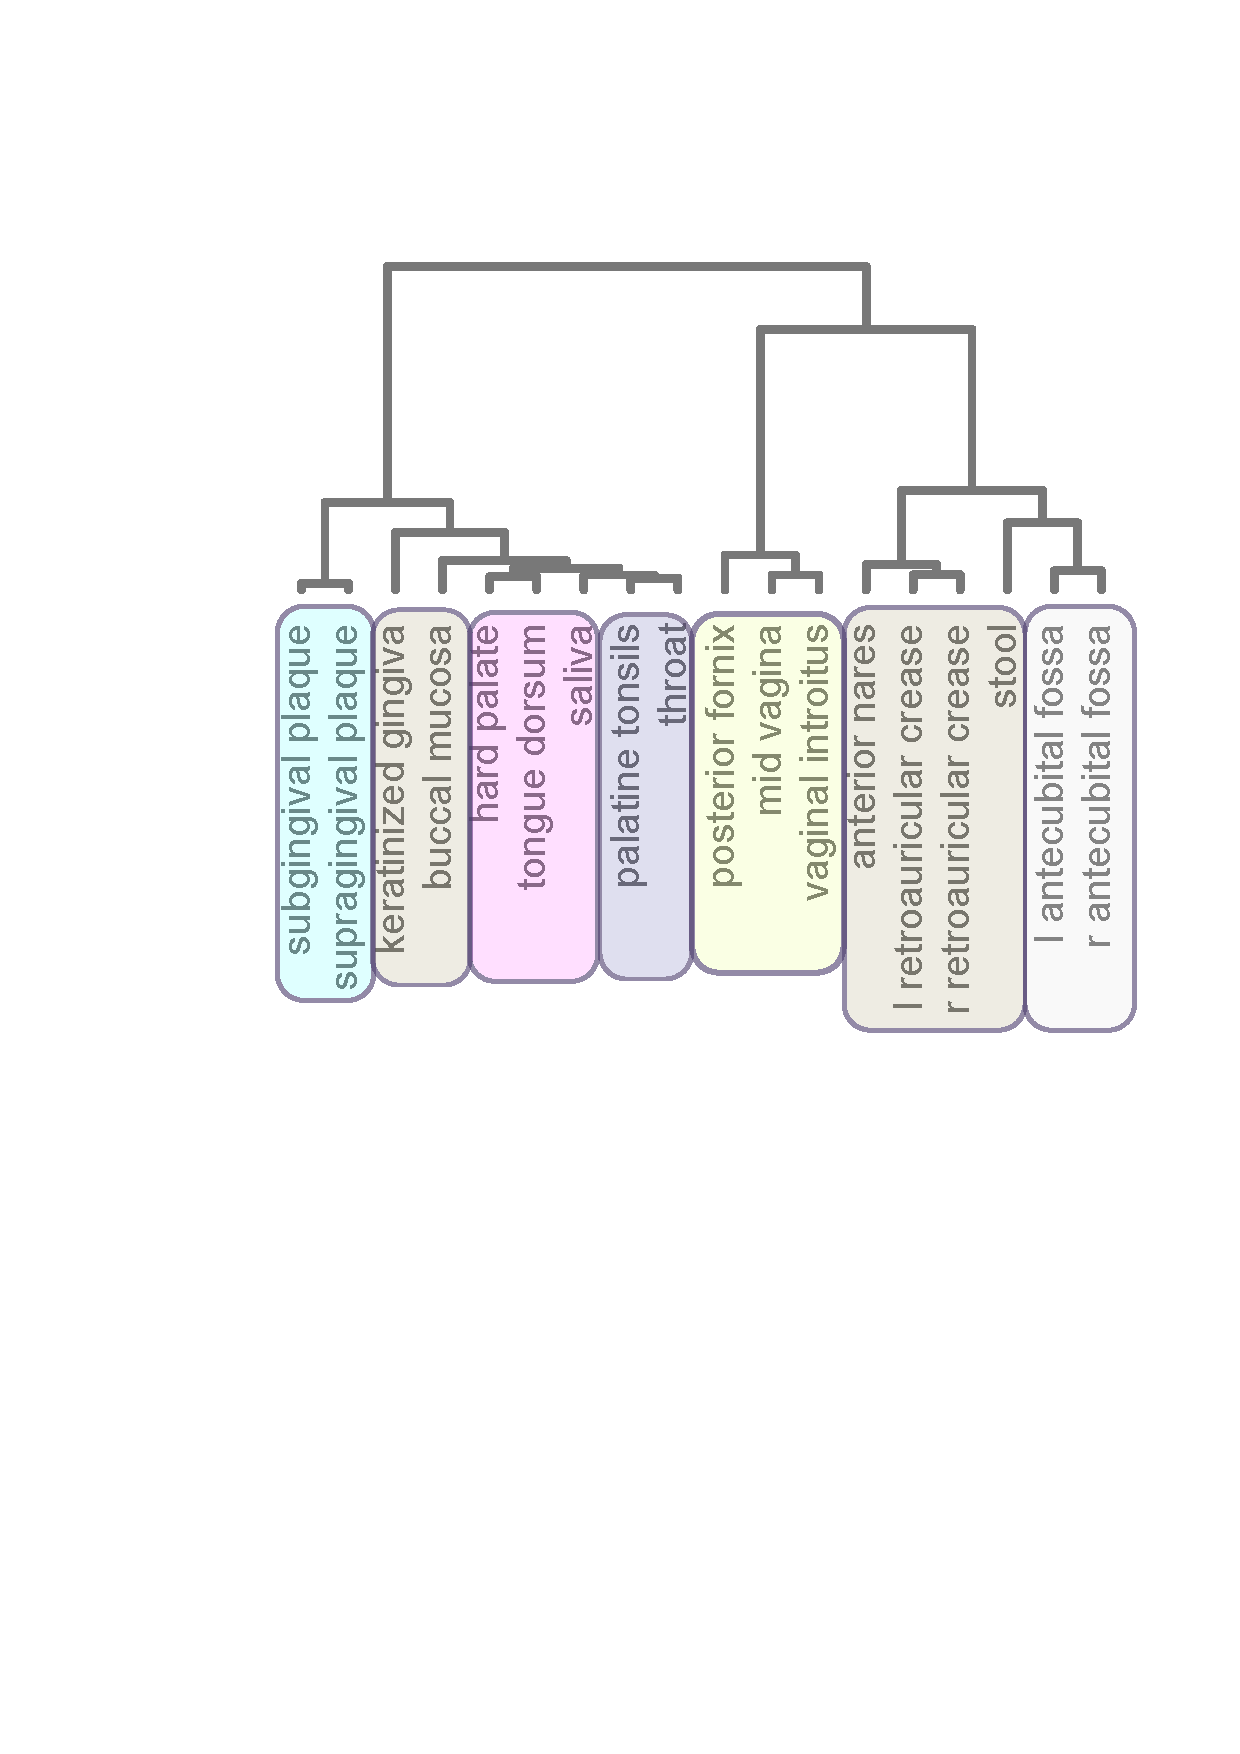
\includegraphics[width=.5\linewidth]{Fig5.pdf}
\caption{{\bf Comparison of sMLSBM on the OTU interaction networks \cite{sparcc} for each of the body sites to a reducibility hierarchy \cite{domen}.} As described in the text, we consider a multiplex network with $L=18$ layers and $N=213$ nodes, which we group here into $S=6$ strata, while the dendrogram was generated by the method employed as the precursor to the reducibility framework. Colored boxes around the leaves of the dendrogram designate the body site to strata assignments obtained with sMLSBM.}
\end{center}
\end{figure*}

\subsection{Generating samples from the fitted sMLSBM}

\indent In Fig.~6, we illustrate network layers for 4 of the 6 strata that we identify to highlight one advantage of having a probabilistic generative model for microbial composition shared in subsets of body sites. Specifically, each row provides information about the network layers and their fitted sMLSBM model for a particular stratum. Each grid in the figure represents the binary adjacency matrix encoding interactions between OTUs: a colored dot at position $(i,j)$ indicates the existence of an edge $(i,j)$ in the corresponding network layer.
%Edges, or a 1 in the adjacency matrix, are colored. 
In the first column of each row is a sample network generated with the learned SBM parameters of that stratum, $\overline{{\boldsymbol \pi}}^{s}$ and $\overline{{\bf Z}^{s}}$. Columns 2 and 3 show two representative network layers within the stratum. Note that while some strata have more than two members, for illustrative purposes we only show two example layers. 
It is easy to see the very similar block structure between all networks in a given row, corroborating the usefulness of the sMLSBM approach. Finally, we highlight the usefulness of fitting sMLSBM to this multilayer network as each stratum
 elucidates a mechanistic understanding of the relationship between groups of OTUs, which could inspire further biological understanding or inquiry. 

\begin{figure}
\begin{center}
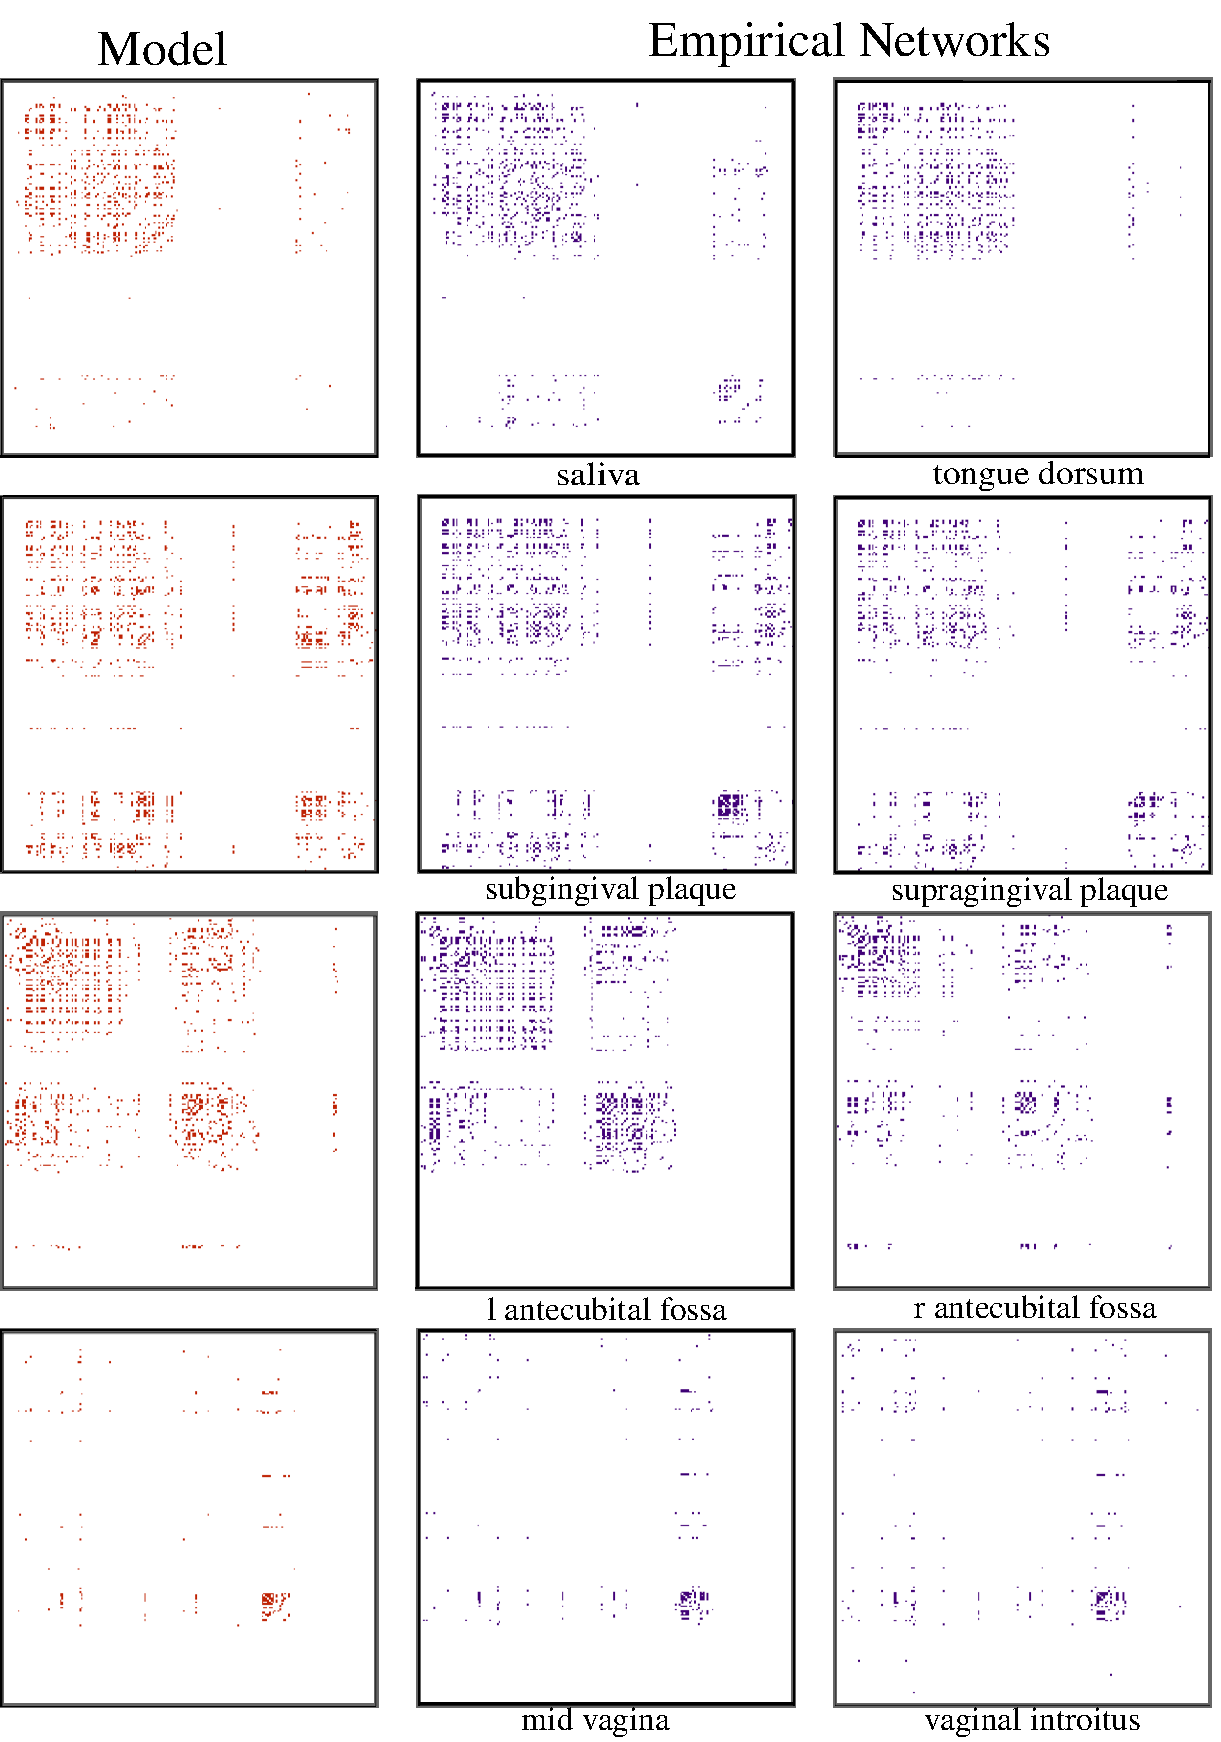
\includegraphics[width=.6\linewidth]{Fig6_Dec15.pdf}
\caption{{\bf Visualization of Strata in SparCC Networks.} We visualize the adjacency matrices for SparCC networks that encode microbiome interactions at body sites. In each panel, a colored dot at position $(i,j)$ indicates the existence of an edge $(i,j)$ in the corresponding network layer. The four rows correspond to four different strata. In column 1, we show a sample network generated from the SBM parameters, $\overline{{\boldsymbol \pi}^{s}}$ and $\overline{{\bf Z}^{s}}$, that we inferred for that stratum. In Columns 2 and 3, we show SparCC networks from that particular stratum. Note the strong similarity across each row.}
\end{center}
\end{figure}

\section{Concluding remarks for sMLSBM}

\indent 
We developed a novel model for multilayer stochastic block models (MLSBMs) and an associated algorithm to jointly partition layers into strata and nodes into communities. Our model assumes that layers belonging to a stratum have community structure following the same underlying SBM. To fit sMLSBM to a multilayer network, and more-specifically, a multiplex network, we iteratively alternate between rearranging layer-to-strata assignments and updating the model parameters for each stratum. Having multiple networks within a stratum---hence multiple realizations from some underlying model---helps to make inference more accurate. Particularly, more accurate assignments of nodes-to-communities within a stratum leads to improved estimation of SBM probability parameters, and vice versa. 
We have shown for multiplex networks with several strata (e.g., see Fig.~3) that inaccuracies can arise if one attempts to fit a single SBM to the network or study the network layers in isolation.
%If layers from different models were all considered to have arisen from the same SBM, both the community memberships and SBM parameters used to represent each layer would be noisier and inaccurate. 
In contrast, our model allows for an understanding of the similarities between layers in a network, in terms of their community structure. 
%
\\\indent
The ability to identify strata within collections of network layers holds promise in numerous applications. 
One motivating application is network reducibility, whereby one compresses a multilayer network by aggregating similar layers \cite{domen}. We stress that although reducibility is a closely related pursuit, it is fundamentally different from our co-clustering pursuit of simultaneously identifying communities and strata. In particular, our approach does not provide a method for aggregating layers. Instead, sMLSBM compresses the network information in the sense that the learned SBM parameters represent a consensus for each stratum, and those consensus parameters can be used to generate a representative sample network for that stratum. For applications in which layer aggregation is sought, there are a variety of ways to aggregate layers in a strata. See, for example, Ref.~\cite{taylor2015enhanced}, where the authors explore the effects on community structure for different aggregation methods. We highlight that the sMLSBM modeling approach is appropriate in situations where one seeks a generative model for community structure, and it may be particularly appropriate when application-specific evidence suggests that subsets of networks have characteristic differences in community structure.
%
\\\indent Our comparison of sMLSBM to the reducibility method of Ref.~\cite{domen} (see Fig.~5) for the application of studying microbial interaction networks reveals several extensions to sMLSBM that could make the approach more accurate and applicable to a wider range of applications. 
First, the reducibility method \cite{domen} does not require networks to be undirected and unweighted, and it could be quite useful to extend the sMLSBM framework to
%since the pairwise distance between networks used there is based on spectral properties. Extensions to 
weighted and directed networks following the extensions for single-layer SBMs, as developed in \cite{weightSBM} and \cite{sbmdirect}, respectively. 
%We note several additional} extensions to sMLSBM that could make the approach more accurate and applicable to a wider range of applications. 
It would also be useful to extend to degree-corrected and overlapping (i.e., mixed-membership) communities \cite{degreecorrectSBM}, as well as mixed membership of layers into strata.
%, could be quite useful. 
%
%
%\\\indent 
Additionally, the Human Microbiome example reveals some interesting biological questions that could facilitate the development of more advanced network tools. To construct the multilayer network, negative edges were thresholded away; however, antagonistic relationships between microbes are known to be important \cite{antagonism}. Thus, it would be useful to develop a signed version of sMLSBM that allows edges to be either positive or negative. \\
\indent The rise of a greater number of multilayer network datasets is providing the need for additional tools for the construction and analysis of such networks. The sMLSBM provides a new method to find signal in inherently noisy and complex network data. 

\section{Detectability in a single stratum}
The development of sMLSBM motivated the analysis for how multiple layers can be collectively used to more accurately learn SBM model parameters in the single stratum case. That is, given a collection of sparse networks from a multilayer stochastic block model with one stratum, how can the layers most accurately be combined to give the most accurate definition of community structure. We investigate these questions in \emph{Enhanced detectability of community structure in multilayer networks through layer aggregation} \cite{taylor2015enhanced}. In particular, we studied the detectability limitations of the stochastic block model for a multilayer network with 1 stratum using random matrix theory techniques. 

\subsection{Investigating detectability in a multilayer network}
Community structure detectability has gained considerable attention \cite{detect20,detect21,detect22,detect23,detect24,detect25} with a hope of being able to identify properties of networks and their corresponding adjacency matrices that reveal how prominent or easy-to-find the community structure is. A network with detectable community structure is thought to be one where multiple community detection algorithms would agree on common groups, and that nodes are not just being assigned to communities randomly, but instead exhibit straight-forward clustering patterns. Applying a community detection algorithm to a network with undetectable community structure might be dramatically different between algorithms, or may assign nodes to the biggest community or even all to the same community. It is particularly interesting to investigate this question in relation to a multilayer stochastic block model because we can generate samples from various models with different parameters and see if the community partition of the network agrees with the specified model. Previous work has previously been explored in networks with degree heterogeneity \cite{detectDegreeHetero}, hierarchical structure \cite{peixotoHierarchAttribute,HierarchAttl}, and in temporal networks \cite{detectTemporal}, but not characterized in multilayer networks. \\
\indent To study this in multilayer networks, we use random matrix theory to study a multilayer network generated from a stochastic block model, and enumerate ways that these layers can be \emph{aggregated} or combined to most improve community structure. We show that the detectability limit vanishes with an increasing number of layers, $L$, and decays as $O(L^{-1/2})$ when we aggregate the the network layers, by taking the sum of their adjacency matrices. Further, we also explore the detectability limits of this aggregated summation of adjacency matrices  that are thresholded to a binary adjacency matrix according to some value, $\tilde{L}$.  

\subsection{Studying detectability in two block networks}
In this work, we study a 2 block multilayer stochastic block model. As seen in previous sections, each network layer has the same set of $N$ nodes and parameterized by an $N$-length vector, ${\bf z}$ specifying the node-to-community assignments and a $2 \times 2$ community probability connectivity matrix, ${\boldsymbol \theta}$. Further, we assume that the between probability connection probability is denoted by $p_{out}$, and that $\pi_{1,2}-\pi_{2,1}=p_{out}$. Similarly, we denote the within-community probability as $p_{in}$, so that $\pi_{1,1}-\pi_{2,2}=p_{in}$ Previous work has shown that for the large network limit, as $N \rightarrow \infty$, there is a solution to the detectability limit \cite{detect23,detect24}, characterized by the solution curve $(\Delta^{*},\rho)$ to 

\begin{equation}
\label{detectEquation}
N\Delta=\sqrt{4N\rho},
\end{equation} 

where $\Delta=p_{in}-p_{out} is the difference in probability and $\rho=(p_{in}+p_{out}/2 is the mean edge probability. For a given value of $\rho$, the communities are only detectable (or correctly characterized) if $\Delta > \Delta^{*}$. Equation \ref{detectEquation} was derived for sparse networks (i.e. constrant $\rho N$ so that $\rho=O(N^{-1})$) and was obtained using both a Bayesian analysis \cite{detect23} and random matrix theory \cite{detect24}.\\
\indent In this work , we study the behavior of $\Delta^{*}$ for two methods of aggregating layers within a multilayer network of $L$ layers, which we denote $\mathcal{L}$. We define the \emph{summation} network, $\bar{\bf A}=\sum_{l \in \mathcal{L}${\bf A}^{l}. Note that, ${\bf A}^{l}$ gives the adjacency matrix for network layer, $l$. 

\subsection{Using random matrix theory to study detectability}


\chapter{Network compression for community detection with super nodes}
\section{Super pixel pre-processing of images}
\section{Super node pre-processing for networks}
\section{2-Core decomposition approach for selecting seeds as community centers}
\section{Creating a super node network representaion}
\section{Social network data examples}
\section{Benefits of a compressed representation: run time, variability, neighborhood smoothing}

\chapter{An attributed stochastic block model}
\section{Examples of attributed networks}
\section{Models and inference for attributed networks}
\section{Alignment of attributes with communities}
\section{Approaches to an attributed stochastic block model}
\section{A model of conditional independence between attributes and connectivity}
\section{Learning the model parameters}
\section{Example on a synthetic attributed network}
\section{Detectability limits in attributed networks}
\section{Case studies for attributed networks}
\section{Attributed SBM in link prediction}
\section{Attributed SBM in collaborative filtering}

\chapter{Community detection for understanding burn inhalation injury}


\chapter{Conclusion and future work}


% Bibliography
\clearpage
\phantomsection

{\def\chapter*#1{} % suppress bibliograph header.
\begin{singlespace}
\addcontentsline{toc}{chapter}{BIBLIOGRAPHY}
\begin{center}
\Large \textbf{BIBLIOGRAPHY}
\vspace{17pt}
\end{center}

\bibliographystyle{apalike}
\bibliography{dissBib}
\end{singlespace}
}





\end{document}
